\documentclass[11pt]{article}
\usepackage[T1]{fontenc}
\usepackage{lmodern}
\usepackage{amsmath,amssymb,amsthm,mathtools}
\usepackage[mathscr]{eucal}
\usepackage[margin=1in]{geometry}
\usepackage{microtype}
\usepackage{booktabs,longtable,array}
\usepackage{enumitem}
\usepackage{graphicx}
\usepackage{tikz}
\usetikzlibrary{arrows.meta,positioning,calc,fit,backgrounds}
\usepackage{xcolor}
\definecolor{linkblue}{RGB}{31,67,102}
\usepackage[colorlinks=true,linkcolor=linkblue,citecolor=linkblue,urlcolor=linkblue,
  bookmarksnumbered=true,pdfusetitle]{hyperref}
\usepackage[nameinlink,capitalise,noabbrev]{cleveref}

\newtheorem{theorem}{Theorem}[section]
\newtheorem{lemma}[theorem]{Lemma}
\newtheorem{proposition}[theorem]{Proposition}
\newtheorem{corollary}[theorem]{Corollary}
\theoremstyle{definition}
\newtheorem{definition}[theorem]{Definition}
\theoremstyle{remark}
\newtheorem{remark}[theorem]{Remark}
\numberwithin{equation}{section}

\newcommand{\F}{\mathbb F}
\newcommand{\R}{\mathbb R}
\newcommand{\E}{\mathbb E}
\renewcommand{\P}{\mathbb P}
\newcommand{\1}{\mathbf 1}
\DeclareMathOperator{\Sym}{Sym}
\DeclareMathOperator{\Lag}{Lag}
\DeclareMathOperator{\rank}{rank}
\DeclareMathOperator{\diag}{diag}
\DeclareMathOperator{\Hom}{hom}
\DeclareMathOperator{\Var}{Var}
\DeclareMathOperator{\Cov}{Cov}
\DeclareMathOperator{\TV}{TV}

\setlist{topsep=4pt,itemsep=2pt,parsep=0pt}
\setlength{\emergencystretch}{2em}
\setcounter{tocdepth}{1}
\allowdisplaybreaks[1]
\ifdefined\pdfinfoomitdate\pdfinfoomitdate=1\fi
\ifdefined\pdftrailerid\pdftrailerid{}\fi
\ifdefined\pdfsuppressptexinfo\pdfsuppressptexinfo=15\fi

\title{A counterexample to Sidorenko's conjecture}
\author{OpenAI}
\date{September 23, 2026}

\begin{document}
\maketitle
\begin{abstract}
We disprove Sidorenko's conjecture with a bipartite graph on \(35\) vertices
and \(66\) edges: its homomorphism density in some finite simple graph is
smaller than the conjectured lower bound. The same connected graph also
disproves the forcing conjecture: at one fixed density, asymptotically
matching the edge and pattern densities does not imply quasirandomness.
\end{abstract}
\tableofcontents

\section{Introduction}\label{sec:introduction}

For finite simple undirected graphs \(H\) and \(G\) with
\(|V(G)|\ge1\), write
\[
t(H,G)=\frac{\Hom(H,G)}{|V(G)|^{|V(H)|}},
\qquad
p(G)=\frac{2|E(G)|}{|V(G)|^2},
\]
where \(\Hom(H,G)\) counts every edge-preserving map, including
noninjective maps. Sidorenko's conjecture asserts that
\begin{equation}\label{eq:sidorenko}
t(H,G)\ge p(G)^{|E(H)|}
\end{equation}
whenever \(H\) is bipartite and has at least one edge.
We disprove this conjecture.

\begin{theorem}\label{thm:main}
Let \(H\) be the incidence graph of the \(22\) triples on \(13\) points
in Table~\ref{tab:complex}. This bipartite graph has \(35\) vertices
and \(66\) edges. There is a finite simple undirected graph \(G\)
with at least one edge such that
\[
t(H,G)<p(G)^{66}.
\]
\end{theorem}

We first construct a strict density gap for a finite nonnegative
kernel and then retain it when sampling a finite simple host. This
route specifies \(H\) explicitly and proves existence of \(G\), while
the final density continues to count all homomorphisms.

A finite kernel is a nonnegative function \(W(x,y)\) on two finite
probability spaces. Its mean is the analogue of edge density, and its
\(H\)-density is the expectation of the product of \(W\) over the
incidences of \(H\), with independent samples from the first space at
the point vertices and from the second space at the face vertices.
For a symmetric kernel taking values in \([0,1]\), a simple graph
can be sampled by choosing a label for each host vertex and using the
kernel value as the probability of each edge.

The same pattern has further consequences with distinct density
scopes. Tensor powers make \(t(H,F)/p(F)^{66}\) arbitrarily small,
with the host density allowed to vary. Balanced blow-ups retain a
fixed deficit in injective labeled copies at one positive limiting
edge density. At one fixed \(p\in(0,1)\), a nonconstant symmetric
\([0,1]\)-valued kernel has mean \(p\) and \(H\)-density \(p^{66}\);
sampling gives finite graphs whose edge and \(H\)-densities converge
to these values while their four-cycle density has a limit strictly
greater than \(p^4\).
Corollaries~\ref{cor:amplification} and~\ref{cor:forcing} state these
consequences precisely below.

\subsection*{The negative correlation}

The triple system has \(13\) points and \(22\) faces. Each of its
\(33\) point pairs belongs to exactly two faces. This double
occurrence converts a local sign constraint into a correlation
involving four incidences.

To see the algebra, attach a sign \(\xi_{ij}\) to each chosen active
incidence and an independent uniform sign \(\eta_e\) to each point
pair. The finite-field lemma compares the averaged matrix product with
a sign model having a factor
\(1+c_0\eta_e\xi_{ij}\xi_{kj}\) whenever both incidences of
\(e=\{i,k\}\) on a face \(j\) are active; here
\(c_0\in\{-1,1\}\). If the two faces on \(e\) are \(j,l\), then
\[
 \E_{\eta_e}
 (1+c_0\eta_e\xi_{ij}\xi_{kj})
 (1+c_0\eta_e\xi_{il}\xi_{kl})
 =
 1+\xi_{ij}\xi_{kj}\xi_{il}\xi_{kl}.
\]
A factor used on only one face averages to \(1\). Thus the model
retains the parity of the four incidence signs exactly when both
face occurrences are selected. This is the finite correlation that
the kernel construction turns negative.

The matrix model uses a large fixed even dimension \(D=2r\).
For a symmetric matrix difference over \(\F_q\), with \(q\) an odd
prime, prescribe rank \(r\)
and the determinant sign of the induced nondegenerate quotient form.
Half rank is the key geometric constraint: when the difference
between two point matrices is nonsingular, the two rank-\(r\) images
through a common center are complementary, which relates their
determinant signs. On configurations with nonsingular point
differences, the normalized center integrals approximate the sign
model in averaged \(L^1\), with a uniform bound on the local factors.
A joint estimate shows that the determinant signs on the \(33\) point
pairs are asymptotically independent, supplying the independent
\(\eta_e\) in the limiting sign model.

The kernel uses one independent matrix coordinate for each incidence.
A type names the point or face that a sampled vertex is intended to
represent. At an incident type pair, two choices of active coordinate
set have opposite sign biases. They cancel every nonconstant first
sign moment while retaining a signed overlap moment. Expanding the
parity model assigns a set of selected coordinates to each point
pair. The chosen supports permit exactly one collection of nonempty
pair labels at the intended type assignment, and its product of
overlap moments is negative. Scores obtained from color refinement
make this assignment dominate all other part-preserving type maps,
including maps with repetitions.

The limiting density in one orientation now has a negative correction.
Adding an inactive point type makes that correction occur with a factor
\(\varepsilon^{13}\), while the uncontrolled correction in the
opposite orientation has a factor \(\varepsilon^{22}\). Choosing
\(\varepsilon>0\) sufficiently small and then taking \(q\) sufficiently
large makes the product of the two finite oriented densities less than
one. A crossed product of the rectangular kernel
with its transpose then gives a symmetric kernel with the same strict
deficit.

The remaining issue is the contribution of singular point
differences. Their probability is \(O(q^{-1})\), but the normalized
rank indicators can grow as a power of \(q\), so the weighted
contribution requires a separate bound. The graph
\(\{(v,Xv):v\in\F_q^D\}\) of a symmetric matrix is a Lagrangian
subspace of \(\F_q^D\oplus\F_q^D\) for
\[
 \omega((v,w),(v',w'))=v^{\mathsf T}w'-w^{\mathsf T}v'.
\]
The intersection of two such graphs projects isomorphically onto
the kernel of their difference. Rank defects thereby become
intersection dimensions.

We compare the probability of each point-intersection profile with
the gain from conditioning on its intersections with a face center.
Three partitions of the face set give a global profile bound. If this
first bound does not give decay, a quadratic estimate forces any large
pair intersection to propagate through the connected complex until
the extra separation of one pair makes the profile too costly. The
remaining bounded dimensions reduce, after choosing \(D\), to a
short list of integer equality cases. A final span count gives strict
decay for those cases. The dimension and all finite construction
parameters are fixed before \(q\) tends to infinity; constants in
the \(q\)-estimates may depend on that fixed dimension.

Figure~\ref{fig:proof-overview} summarizes these dependencies.

\begin{figure}[htbp]
\centering
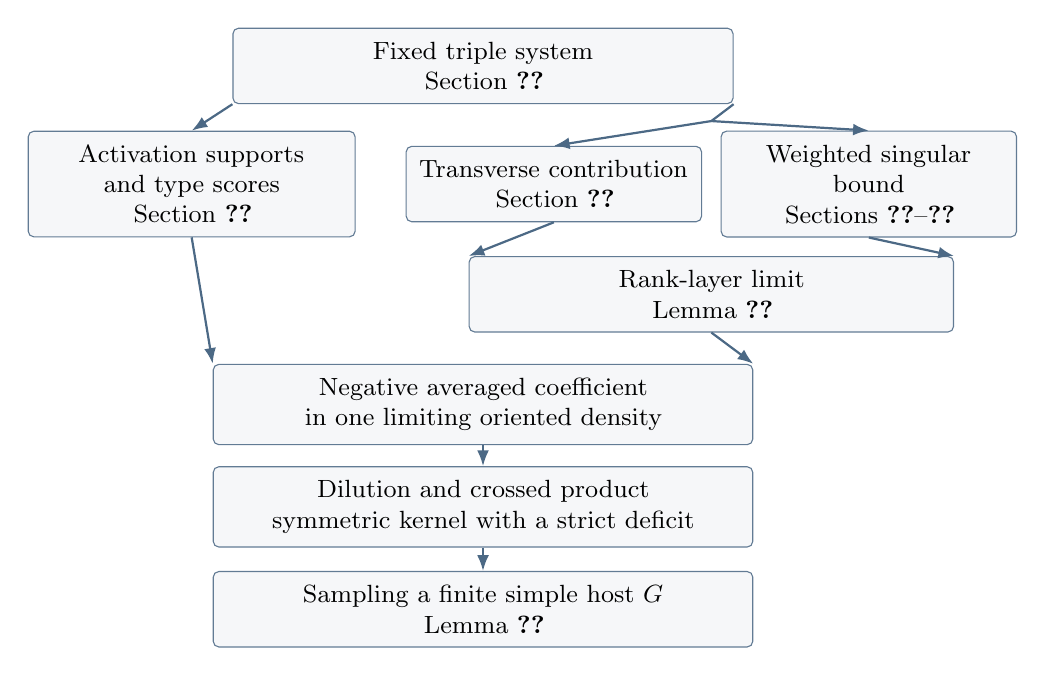
\begin{tikzpicture}[
  font=\small,
  proofbox/.style={draw=linkblue!70,rounded corners=2pt,
    fill=linkblue!4,align=center,inner sep=5pt,text width=3.4cm},
  proofstep/.style={-{Latex[length=2mm]},thick,draw=linkblue!80}]
  \node[proofbox,text width=6.0cm] (complex) at (0,0)
    {Fixed triple system\\Section~\ref{sec:complex}};
  \node[proofbox,text width=3.8cm] (activation) at (-3.7,-1.5)
    {Activation supports\\and type scores\\Section~\ref{sec:kernel}};
  \node[proofbox] (transverse) at (0.9,-1.5)
    {Transverse contribution\\Section~\ref{sec:transverse}};
  \node[proofbox] (tail) at (4.9,-1.5)
    {Weighted singular\\bound\\Sections~\ref{sec:orbits}--\ref{sec:tail}};
  \node[proofbox,text width=5.8cm] (rank) at (2.9,-2.9)
    {Rank-layer limit\\Lemma~\ref{lem:rank-layer}};
  \node[proofbox,text width=6.5cm] (negative) at (0,-4.3)
    {Negative averaged coefficient\\in one limiting oriented density};
  \node[proofbox,text width=6.5cm] (kernel) at (0,-5.6)
    {Dilution and crossed product\\symmetric kernel with a strict deficit};
  \node[proofbox,text width=6.5cm] (host) at (0,-6.9)
    {Sampling a finite simple host $G$\\Lemma~\ref{lem:finite-host}};
  \coordinate (estimatefork) at (2.9,-0.7);
  \draw[proofstep] (complex.south west) -- (activation.north);
  \draw[proofstep] (complex.south east) -- (estimatefork) -- (transverse.north);
  \draw[proofstep] (estimatefork) -- (tail.north);
  \draw[proofstep] (transverse.south) -- (rank.north west);
  \draw[proofstep] (tail.south) -- (rank.north east);
  \draw[proofstep] (activation.south) -- (negative.north west);
  \draw[proofstep] (rank.south) -- (negative.north east);
  \draw[proofstep] (negative) -- (kernel);
  \draw[proofstep] (kernel) -- (host);
\end{tikzpicture}
\caption{Logical dependencies of the counterexample. The fixed triple
system supplies the combinatorial properties used in both branches.
The rank-layer limit realizes the averaged coefficient made negative
by the finite activation construction. Section~\ref{sec:kernel}
constructs the kernel and transfers its strict deficit to a finite
simple host assuming Lemma~\ref{lem:rank-layer};
Sections~\ref{sec:transverse}--\ref{sec:tail} then prove that input.}
\label{fig:proof-overview}
\end{figure}


\subsection*{History and relation to positive results}

The conjecture grew out of questions about supersaturation: how many
copies of a fixed bipartite graph must occur once the host has many
edges? In a related study of graphcopy functions, Erd\H{o}s,
Lov\'asz, and Spencer distinguished normalized homomorphism and
injective-copy counts and proved their limiting agreement under
increasing host orders~\cite{erdoslovaszspencer1979}.
Simonovits's discussion of degenerate extremal problems placed
supersaturation lower bounds in a general program~\cite{simonovits1984}.
Sidorenko formulated the associated inequalities for functionals of
nonnegative kernels~\cite{sidorenko1991,sidorenko1993}.  In the
homomorphism formulation, the proposed lower bound is the density in
a constant kernel of the same mean.  The insistence on all
homomorphisms is part of this formulation; repeated images of vertices
are allowed.  Theorem~\ref{thm:main} concerns this ordinary graph
inequality.

Trees, even cycles, and complete bipartite graphs are basic positive
examples~\cite{sidorenko1993}. Several methods established broader
classes. Conlon,
Fox, and Sudakov proved the conjecture when one vertex is adjacent to
the entire opposite part, and obtained more general comparisons with
complete bipartite graphs~\cite{conlonfoxsudakov2010}.  A different
approach studies norms derived from homomorphism densities.
Hatami developed the graph-norm approach, recording Szegedy's observation
that weakly norming graphs satisfy Sidorenko's inequality, and proved
stronger subgraph inequalities and the hypercube case~\cite{hatami2010}.
Conlon and Lee constructed weakly norming graphs from finite reflection
groups~\cite{conlonlee2017}.  These results provide stronger inequalities
than the comparison with a single edge and explain why many highly
structured bipartite graphs satisfy the conjecture.

Other proofs assemble a graph from pieces while keeping control of
the associated homomorphism distribution.  Li and Szegedy's logarithmic
calculus, first circulated in 2011, gives gluing results and a class of
reflection trees~\cite{liszegedy2025}.  Szegedy developed an information
theoretic formulation using entropy and conditional
gluing~\cite{szegedy2015entropy}.  Kim, Lee, and Lee proved the conjecture
for tree-arrangeable graphs and for Cartesian products of a Sidorenko
graph with a tree~\cite{kimleelee2016}.  Conlon, Kim, Lee, and Lee
introduced strong tree decompositions and established further
subdivision results~\cite{conlonkimleelee2018}.  More recently, Im,
Li, and Liu treated subdivisions and substitutions by even theta
graphs under a local-density counting hypothesis for the base or suitable
global path-multiplicity conditions~\cite{imliliu2026}.
The gluing and substitution statements impose different structural
conditions on their constituent graphs.

Positive results also depend on how often neighborhoods of a given
size occur. Conlon and Lee proved a divisibility criterion and a
degree-count criterion when one part is regular, and showed that every
bipartite graph has a sufficiently large one-sided blow-up satisfying
the conjecture~\cite{conlonlee2021}. Coregliano subsequently replaced
the divisibility hypothesis with weaker degree-count bounds and
extended the reflection approach through left-cut-percolation and
induced-Sidorenko bigraphs~\cite{coregliano2024}.  A positive result
for a blow-up does not imply the corresponding result for the
original graph.

There are useful reductions of the host space as well. Coregliano and
Razborov proved that, for a fixed pattern, a lower bound by one fixed
positive multiple of the Sidorenko expression on every biregular
bigraphon implies the exact Sidorenko inequality on every bigraphon.
Here biregular means that the
kernel integrals in either variable are constant. They also proved a
reflective tree-decomposition theorem~\cite{coreglianorazborov2021}.
In another direction, Zhao gave a conditional reduction through
conjugacy-class averaging on finite groups and proved an inequality
for one-subdivisions on the resulting conjugacy-averaged bipartite
Cayley kernels~\cite[Theorems~1.3--1.4]{zhao2026conjugacy}.  The averaging monotonicity in the
general reduction is a hypothesis.

The incidence graph used here has parts of sizes $13$ and $22$,
with degrees $4,5,6$ on the first part and degree $3$ on the second.
It therefore has no vertex adjacent to the whole opposite part.
Since it is connected and its first part is not regular, it is not
weakly norming: Hatami's necessary condition requires regularity on
each part~\cite{hatami2010}. Coregliano's sufficient degree-count
hypothesis is not met in either orientation.  On the degree-$3$ side the relevant comparison is
$22<\binom{13}{3}=286$; in the reverse orientation there are only
$3,6,4$ vertices of degrees $4,5,6$, respectively, below the
corresponding thresholds
$\binom{22}{4},\binom{22}{5},\binom{22}{6}$~\cite[Theorem~3.6]{coregliano2024}.
Its minimum degree is $3$, so it is not directly a graph obtained by
the even-path substitutions above, which introduce vertices of
degree $2$.  These observations locate the example relative to
specific positive theorems; the negative inequality is established by
the construction and estimates below.

Finally, the conclusion is compatible with local versions of the
conjecture.  For a bipartite graph with $m$ edges, Lov\'asz proved the
inequality for a mean-one symmetric kernel $W$ satisfying
$\lVert W-1\rVert_\infty\leq 1/(4m)$~\cite[Theorem~5.1]{lovasz2011local}.
He also proved a cut-norm
version under the additional bound $0\leq W\leq2$, with
$\lVert W-1\rVert_\square\leq2^{-8m-2}$~\cite[Theorem~4.1]{lovasz2011local}.
Here the kernels are on $[0,1]^2$, with Lebesgue measure, and
\[
 \lVert F\rVert_\square
 =\sup_{S,T\subseteq[0,1]}
   \left|\int_{S\times T}F(x,y)\,dx\,dy\right|,
\]
where $S,T$ are measurable. Thus the constant kernel has a neighborhood
on which the inequality holds. A finite probability kernel can be
represented on $[0,1]^2$ by a step function whose interval lengths
are its atom probabilities. The mean-one normalization of our final
symmetric kernel, having a strict deficit, cannot satisfy either set
of local hypotheses above. Scaling the kernel into $[0,1]$ preserves
the normalized density comparison.

The construction also uses established geometric and algebraic
frameworks in specific roles. Conditions on the rank and
discriminant sign of a symmetric matrix difference are the relations
in the association scheme of symmetric matrices studied by Huo and
Wan~\cite{huowan1993}; Schmidt records this framework and the exact
counts by rank and sign~\cite[Section~2]{schmidt2015}. Symplectic geometry
provides the elementary Lagrangian and pair-intersection counting
formulas~\cite{taylor1992}.
The joint-sign argument uses the standard quadratic Gauss-sum rank
bound~\cite[Lemma~3.3]{gowerswolf2011}, and the type scores adapt
color refinement~\cite{weisfeilerleman1968,mckay1981}. We rederive
the estimates used here and combine the signed rank-layer correlations
with bounds for their weighted contribution on singular configurations.

\subsection*{Amplification and injective copies}

For a finite simple graph \(F\) of order \(n\ge35\), let
\(\operatorname{Inj}(H,F)\)
count injective edge-preserving maps, with no condition on nonedges,
and write \((n)_{35}=n(n-1)\cdots(n-34)\). At ordinary edge density
\(d=|E(F)|/\binom n2\), the labeled random-graph benchmark is
\((n)_{35}d^{66}\), the expected count in \(G(n,d)\).

\begin{corollary}[Amplification and injective supersaturation]
\label{cor:amplification}
For the same graph \(H\) as in Theorem~\ref{thm:main}, the following
hold.
\begin{enumerate}[label=(\roman*)]
\item For every \(c>0\), there is a finite simple undirected graph
\(F\) with \(p(F)>0\) such that
\[
t(H,F)<c\,p(F)^{66}.
\]
\item There are \(p_*\in(0,1)\), \(\delta_*>0\), and finite simple
undirected graphs \(F_s\) of orders \(n_s\to\infty\) for which
\(d_s=|E(F_s)|/\binom{n_s}{2}\to p_*\) and, for all sufficiently
large \(s\),
\[
\operatorname{Inj}(H,F_s)
\le(1-\delta_*)(n_s)_{35}d_s^{66}.
\]
\end{enumerate}
\end{corollary}

The proof in Section~\ref{sec:consequences} uses tensor powers and
balanced blow-ups of a single host from Theorem~\ref{thm:main}.

Part (ii) contradicts the injective Erd\H{o}s--Simonovits
random-graph benchmark described in
\cite[Section~1]{conlonfoxsudakov2010}: the sequence has one positive
limiting density, so it eventually satisfies \(d_s>n_s^{-\gamma}\)
for every fixed \(\gamma>0\), while retaining a fixed deficit.

\subsection*{A consequence for the forcing conjecture}

Fix \(0<p<1\). A graph \(F\) with \(m\) edges is \emph{\(p\)-forcing}
if every sequence of finite simple graphs \(G_n\) with
\(|V(G_n)|\to\infty\), \(p(G_n)\to p\), and
\(t(F,G_n)\to p^m\) is quasirandom of density \(p\): for every fixed
finite simple graph \(J\), one has
\(t(J,G_n)\to p^{|E(J)|}\). It is \emph{forcing} if it is
\(p\)-forcing for every \(p\in(0,1)\). The classical edge-and-four-cycle
characterization of quasirandomness is due to Chung, Graham, and
Wilson~\cite{chunggrahamwilson1989}. Skokan and Thoma studied which
bipartite patterns can replace the four-cycle~\cite{skokanthoma2004}.
Using this asymptotic formulation and following their question,
Conlon, Fox, and Sudakov formulate the forcing conjecture: a graph is forcing if and
only if it is bipartite and contains a cycle
\cite[Section~1, equation~(2) and Conjecture~2]{conlonfoxsudakov2010}.

For a symmetric \([0,1]\)-valued kernel \(W\) on a probability space,
write
\[
t(F,W)=\E\prod_{uv\in E(F)}W(X_u,X_v),
\]
where the \(X_v\) are independent samples. In particular,
\(t(K_2,W)=\E W\). We identify each finite probability kernel below
with its step graphon on \([0,1]\).

\begin{corollary}[Failure of the forcing conjecture]
\label{cor:forcing}
For the same connected bipartite graph \(H\) of
Theorem~\ref{thm:main}, there are \(p\in(0,1)\) and a nonconstant
graphon \(W\) such that
\[
t(K_2,W)=p,\qquad t(H,W)=p^{66}.
\]
Consequently, \(H\) is not \(p\)-forcing at this density and hence is
not forcing, despite being bipartite and containing a cycle.
\end{corollary}

Section~\ref{sec:consequences} interpolates between finite kernels of
the same mean to obtain the exact graphon equality, then uses independent
sampling to obtain a sequence of finite graphs with the stated limiting
densities.
Conlon, Fox, and Sudakov note that the forcing conjecture is stronger
than Sidorenko's conjecture~\cite[Section~1]{conlonfoxsudakov2010};
the interpolation gives a concrete witness for this graph at one density.

\subsection*{Organization and conventions}

Section~\ref{sec:complex} gives the triple system and verifies its
finite properties. Section~\ref{sec:kernel} states
Lemma~\ref{lem:rank-layer} and uses it to prove
Theorem~\ref{thm:main}. The next four sections prove that lemma:
Section~\ref{sec:transverse} treats transverse matrices;
Section~\ref{sec:orbits} gives the Lagrangian orbit counts;
Section~\ref{sec:planted} bounds the local gains; and
Section~\ref{sec:tail} proves strict decay of the singular
contribution. Section~\ref{sec:consequences} then proves the amplification,
injective-copy and forcing consequences stated above.

All probability spaces used in our construction are finite. Expectations
refer to the indicated independent samples, except where a
conditional law is specified. Empty products equal \(1\).
The field size \(q\) tends to infinity through odd primes. Every
such limit is taken after fixing the dimension and all finite
construction parameters. Dependence on \(D\) in the constants of
these \(q\)-asymptotic estimates is allowed; bounds used to choose
\(D\) will explicitly be uniform in \(D\).

\section{The finite complex}
\label{sec:complex}

We specify the fixed triple system and certify the properties used in
both the kernel construction and the singular-tail bound.

Let $I=\{0,\ldots,12\}$ and $J=\{0,\ldots,21\}$. Associate to
each $j\in J$ the three-element subset of $I$ in Table~\ref{tab:complex};
we call these subsets \emph{faces} and also denote them by $j$.
Let $E$ be the set of unordered point pairs contained in a face.
The graph used throughout the paper is the incidence graph
\[
 H=(I\sqcup J,\mathscr C),\qquad
 \mathscr C=\{(i,j):i\in j\}.
\]
The copies of $I$ and $J$ in this disjoint union are distinct even when
their numerical labels agree. We call an incidence $(i,j)$ a
\emph{corner}. Thus $H$ has $35$ vertices and $66$ edges.

\begin{table}[htbp]
\centering
\small
\setlength{\tabcolsep}{7pt}
\begin{tabular}{c@{\qquad}ccc@{\qquad}ccc@{\qquad}c}
\toprule
Face&\multicolumn{3}{c}{Points}&\multicolumn{3}{c}{Opposite face}&Bits\\
 $j$&$i_1$&$i_2$&$i_3$&$j_{12}$&$j_{13}$&$j_{23}$&\\
\midrule
0 &0&1&3   &1&2&4   &000\\
1 &0&1&9   &0&3&7   &010\\
2 &0&2&3   &3&0&8   &001\\
3 &0&2&9   &2&1&9   &110\\
4 &1&3&10  &0&5&11  &001\\
5 &1&7&10  &6&4&16  &000\\
6 &1&7&12  &5&7&18  &100\\
7 &1&9&12  &1&6&21  &110\\
8 &2&3&4   &2&9&10  &101\\
9 &2&4&9   &8&3&12  &100\\
10&3&4&11  &8&11&13 &111\\
11&3&10&11 &4&10&17 &101\\
12&4&8&9   &13&9&21 &101\\
13&4&8&11  &12&10&19&011\\
14&5&6&7   &15&16&18&000\\
15&5&6&11  &14&17&19&110\\
16&5&7&10  &14&17&5 &010\\
17&5&10&11 &16&15&11&111\\
18&6&7&12  &14&20&6 &001\\
19&6&8&11  &20&15&13&010\\
20&6&8&12  &19&18&21&011\\
21&8&9&12  &12&20&7 &111\\
\bottomrule
\end{tabular}
\caption{The faces of the complex. The entry $j_{ab}$ is the other
face containing $\{i_a,i_b\}$. Bit positions are read from left to right.}
\label{tab:complex}
\end{table}

Join two faces when they share a pair. This defines the
\emph{face-neighbor graph}. For a pair $e\in E$, define
\begin{equation}
 a_e=\frac{1}{3}\#\{\text{bit positions at which the two faces on $e$
 differ}\}.
 \label{eq:complex-separation}
\end{equation}

Color refinement starts with a separate color for each part of $H$.
A refinement step replaces a vertex's color by the ordered pair
consisting of its old color and the histogram of its neighbors' old
colors. This is the classical color-refinement procedure; see
Weisfeiler and Leman~\cite{weisfeilerleman1968} and
McKay~\cite[Sections~2.3--2.6]{mckay1981} for its equitable-partition interpretation.

\begin{proposition}
\label{prop:complex}
The complex has the following properties.
\begin{enumerate}
\item Every pair in $E$ lies in exactly two faces, $|E|=33$, and the
face-neighbor graph is connected.
\item For each bit position, each of its two classes consists of
$11$ faces covering all $13$ points. Each class has an ordering in
which every face after the first shares a pair with an earlier face
and introduces exactly one new point.
\item Every $a_e$ is at least $1/3$, and some $a_e$ is greater than
$1/3$.
\item Color refinement of $H$, starting with a separate color for each
part, eventually gives distinct colors to all vertices within either
part.
\end{enumerate}
\end{proposition}

\begin{proof}
The neighbor entries in Table~\ref{tab:complex} pair the $66$
face--pair incidences into $33$ reciprocal pairs. Comparing the
triples in each indicated pair shows that their common point pair is
exactly the one specified. No other face contains that pair, as is
also checked by the same table.

Table~\ref{tab:complex-orders} gives all six orders and their
new-point certificates for the second assertion.

\begin{table}[htbp]
\centering
\small
\setlength{\tabcolsep}{5pt}
\begin{tabular}{cc@{\qquad}ll}
\toprule
\multicolumn{2}{c}{Bit class}&Face order&New points after the first face\\
Position&Value&&\\
\midrule
1&0&$0,1,2,4,5,16,14,18,20,19,13$
 &$9,2,10,7,5,6,12,8,11,4$\\
1&1&$3,9,8,10,11,17,15,12,21,7,6$
 &$4,3,11,10,5,6,8,12,1,7$\\
\addlinespace
2&0&$0,2,8,9,12,4,11,5,6,18,14$
 &$2,4,9,8,10,11,7,12,6,5$\\
2&1&$1,3,7,21,20,19,13,10,15,17,16$
 &$2,12,8,6,11,4,3,5,10,7$\\
\addlinespace
3&0&$0,1,3,9,7,6,5,16,14,15,19$
 &$9,2,4,12,7,10,5,6,11,8$\\
3&1&$2,8,10,11,4,17,13,12,21,20,18$
 &$4,11,10,1,5,8,9,12,6,7$\\
\bottomrule
\end{tabular}
\caption{An exposure order for each bit class. Every face after the
first shares a pair with an earlier face and introduces the
corresponding point in the last column. Bit positions are read from
left to right in Table~\ref{tab:complex}.}
\label{tab:complex-orders}
\end{table}

The root face contributes its three points, and these ten new points
give all of $I$ in each case. The shared-pair condition follows from
the neighbor columns of Table~\ref{tab:complex}. Thus every bit class
is connected. The first two classes are joined, for example, by
faces $2$ and $3$, so the whole face-neighbor graph is connected.
Inspection of the bit labels gives separation in at least one
position on every pair. The pair $\{0,2\}$ has adjacent labels
$001$ and $110$, so in fact $a_{\{0,2\}}=1$.

It remains to verify the color-refinement assertion. First consider
the point graph $(I,E)$. Its point degrees $d_i$ and the numbers
$n_4(i),n_5(i),n_6(i)$ of neighbors of degrees $4,5,6$ are as follows:
\begin{equation}
\begin{array}{c|c|ccc@{\qquad}c|c|ccc}
i&d_i&n_4&n_5&n_6&i&d_i&n_4&n_5&n_6\\\hline
0&4&1&0&3&7&5&1&3&1\\
1&6&1&3&2&8&5&0&3&2\\
2&4&1&1&2&9&6&2&3&1\\
3&6&2&2&2&10&5&1&1&3\\
4&5&1&1&3&11&6&1&4&1\\
5&4&0&3&1&12&5&0&3&2\\
6&5&1&3&1&&&&&
\end{array}
\label{eq:complex-colors}
\end{equation}
Only the pairs $\{4,10\}$, $\{6,7\}$, and $\{8,12\}$ have
equal signatures in Equation~\eqref{eq:complex-colors}. The first is
separated by adjacency to the already distinguished point $2$:
$4$ is adjacent to $2$, whereas $10$ is not. The other two are
separated by adjacency to the already distinguished point $11$:
$6$ and $8$ are adjacent to $11$, whereas $7$ and $12$ are not.
Hence refinement on the point graph is discrete.

This point refinement can be recovered from incidence refinement.
The degree of $i$ in $H$ equals $d_i$: counting other points in its
incident faces gives twice each neighbor in $(I,E)$. More generally,
suppose the current incidence color of every point determines a point
coloring \(\ell\) through a fixed projection. One further incidence
step determines, at each face \(j\), the color-indexed histogram
\[
 m_j(\gamma)=\#\{k\in j:\ell(k)=\gamma\}.
\]
The next step determines the multiset of these histograms over the
faces incident to each point. For every color
\(\gamma\), this gives
\[
 \sum_{j\ni i}
 \left(m_j(\gamma)-\1_{\{\gamma=\ell(i)\}}\right)
 =2\,\#\{k:\{i,k\}\in E,\ \ell(k)=\gamma\}.
\]
The subtraction removes only the occurrence of \(i\) in each face,
even when other points have the same color. Each neighbor is counted
twice because its pair with \(i\) lies in two faces. Dividing by two
therefore recovers the point neighbor-color histogram.
Thus two incidence steps recover each further point refinement step.
After the point colors are discrete, one more step distinguishes all
faces, since their three-element point sets are distinct. This proves
the last assertion without any assumption about a chosen refinement
implementation.
\end{proof}

\section{Constructing a negative kernel correlation}
\label{sec:kernel}

This section reduces Theorem~\ref{thm:main} to a finite-field counting
lemma. We first state that lemma, then construct a nonnegative kernel
whose homomorphism density is too small. All probability spaces in
the construction are finite; their atom probabilities need not be
rational.

\subsection{The rank-layer model}

Let $q$ be an odd prime, let $\chi:\F_q\to\{0,1,-1\}$ be the
quadratic character with $\chi(0)=0$, and let $\mathcal S_D$ be the
space of symmetric $D$-by-$D$ matrices over $\F_q$, equipped with
uniform probability. For a symmetric matrix of positive rank, its
\emph{sign} is the quadratic character of the determinant of its
induced nondegenerate symmetric form on the quotient by the radical.
A change of basis multiplies this determinant by a square, so the
sign is well defined. Fix a positive even dimension $D=2r$ and set
\begin{equation}
 K_\xi(Z)=
 \frac{\1_{\{\rank Z=r,\ \operatorname{sign}(Z)=\xi\}}}
 {\P_{Z'\in\mathcal S_D}(\rank Z'=r,\ \operatorname{sign}(Z')=\xi)},
 \qquad \xi\in\{1,-1\},\qquad c_0=\chi((-1)^r).
 \label{eq:kernel-rank-definition}
\end{equation}
Both denominators are positive: diagonal matrices realize either
nonzero determinant square class in rank $r$. In particular,
$K_\xi\ge0$ and $\E K_\xi=1$.

\begin{lemma}[Rank-layer limit]
\label{lem:rank-layer}
There is an integer $D_0$ such that, for every fixed even $D\ge D_0$,
the following assertion holds as $q$ tends to infinity through odd
primes. Let $X_i$, $i\in I$, and $Y_j$, $j\in J$, be independent
uniform elements of $\mathcal S_D$. For every set
$B\subseteq\mathscr C$ and every choice of signs
$\xi_{ij}\in\{1,-1\}$ on $B$,
\begin{equation}
 \E\prod_{(i,j)\in B}K_{\xi_{ij}}(X_i-Y_j)
 =\E_\eta\prod_{j\in J}
 \prod_{\substack{e=\{i,k\}\subset j\\(i,j),(k,j)\in B}}
 \bigl(1+c_0\eta_e\xi_{ij}\xi_{kj}\bigr)+o(1),
 \label{eq:rank-layer}
\end{equation}
where the $\eta_e$, $e\in E$, are independent uniform signs. The error
is uniform over all such $B$ and sign choices. The same assertion
holds with $Y_j-X_i$ in place of $X_i-Y_j$.
\end{lemma}

The averaging on the right has a useful exact form. For
\(e=\{v,w\}\in E\), let \(j,l\) be its two faces and put
\begin{equation}
 U_e=\{(v,j),(w,j),(v,l),(w,l)\}\subseteq\mathscr C.
 \label{eq:kernel-four-corners}
\end{equation}
Write \(\xi_\kappa=\xi_{ij}\) for \(\kappa=(i,j)\in B\).
If only one of the two face factors on \(e\) is present, its average
over \(\eta_e\) is \(1\). If both are present, their average is
\(1+\prod_{\kappa\in U_e}\xi_\kappa\), since \(c_0^2=1\).
Independence of the \(\eta_e\) therefore gives
\begin{equation}
 \E_\eta\prod_{j\in J}
 \prod_{\substack{e=\{i,k\}\subset j\\(i,j),(k,j)\in B}}
 (1+c_0\eta_e\xi_{ij}\xi_{kj})
 =
 \prod_{\substack{e\in E\\U_e\subseteq B}}
 \left(1+\prod_{\kappa\in U_e}\xi_\kappa\right).
 \label{eq:kernel-parity-model}
\end{equation}
Thus every fully active pair tests the parity of its four incidence
signs, contributing \(0\) or \(2\). This is an identity for the
integrated sign model in Equation~\eqref{eq:rank-layer}. The
quantification over \(B\) is needed because each coordinate in the
activation construction below selects its own active incidences.

The proof of Lemma~\ref{lem:rank-layer} occupies
Sections~\ref{sec:transverse}--\ref{sec:tail}.
The dimension is fixed before the prime tends to infinity; uniformity
in $B$ and the signs then concerns a fixed finite family. For the
assertion with reversed matrix differences, negation multiplies the sign of a rank-$r$ matrix by
$c_0$ and bijects the corresponding layers, whence
$K_\xi(-Z)=K_{c_0\xi}(Z)$. Replacing every incidence sign by
$c_0\xi_{ij}$ leaves each sign product on the right of
Equation~\eqref{eq:rank-layer} unchanged.

For a kernel $W:\mathcal X\times\mathcal Y\to[0,\infty)$ on two
finite probability spaces, write
\begin{equation}
 t_{I,J}(W)=\E\prod_{(i,j)\in\mathscr C}W(x_i,y_j),
 \qquad W^\top(y,x)=W(x,y),
 \label{eq:kernel-bipartite-density}
\end{equation}
where all $x_i\in\mathcal X$ and $y_j\in\mathcal Y$ are sampled
independently. Thus $t_{I,J}(W^\top)$ samples the $I$-vertices from
$\mathcal Y$ and the $J$-vertices from $\mathcal X$.

For a symmetric kernel $U:\Omega\times\Omega\to[0,\infty)$ on one
finite probability space, write $t(H,U)=t_{I,J}(U)$, with every vertex
sampled independently from $\Omega$; sampled labels may coincide.

\subsection{Activation laws and the coordinate expansion}

A type records which point or face of the fixed complex a sampled
vertex is intended to represent. Independent matrix coordinates carry
separate copies of the rank-layer model, and an activation law chooses
which copies occur at a pair of types. We first leave these finite
choices arbitrary and derive their contribution to the density.

Let $\mathcal A,\mathcal B$ be finite type sets, with probability
distributions $\pi,\nu$, and let $\mathcal K$ be a fixed finite
coordinate set. Use the spaces
\[
 \mathcal X=\mathcal A\times\mathcal S_D^{\mathcal K},\qquad
 \mathcal Y=\mathcal B\times\mathcal S_D^{\mathcal K},
\]
with the type distributions just specified and all matrix coordinates
independent and uniform. For each $(a,b)\in\mathcal A\times\mathcal B$,
choose a probability law on a subset $S\subseteq\mathcal K$ and signs
$(\xi_\kappa)_{\kappa\in S}$. Define
\begin{equation}
 W_q\bigl((a,x),(b,y)\bigr)
 =\E_{S,\xi\mid a,b}\prod_{\kappa\in S}
 K_{\xi_\kappa}(x^\kappa-y^\kappa).
 \label{eq:kernel-activation}
\end{equation}
An empty product is one. For fixed types, averaging over the matrices
gives one, since each difference is uniform and distinct coordinates
are independent. Therefore $\E W_q=1$, for every $q$.

For $\alpha\subseteq\mathcal K$ put
\[
 \phi_\alpha(S,\xi)=
 \1_{\{\alpha\subseteq S\}}\prod_{\kappa\in\alpha}\xi_\kappa,
 \qquad
 A_{ab}(\alpha,\beta)=\E_{S,\xi\mid a,b}\phi_\alpha\phi_\beta.
\]
Here $\phi_\alpha$ is defined to be zero when $\alpha\not\subseteq S$;
in particular $\phi_\varnothing=1$. We will impose the moment condition
\begin{equation}
 \E_{S,\xi\mid a,b}\phi_\alpha=0
 \quad\text{for every $a,b$ and every nonempty $\alpha$.}
 \label{eq:kernel-zero-moments}
\end{equation}
If $\alpha\cap\beta=\varnothing$, then
$\phi_\alpha\phi_\beta=\phi_{\alpha\cup\beta}$, so
\begin{equation}
 A_{ab}(\alpha,\beta)=0
 \quad\text{if $\alpha\cap\beta=\varnothing$ and
 $\alpha\cup\beta\ne\varnothing$.}
 \label{eq:kernel-disjoint-zero}
\end{equation}

At a corner $(i,j)$, let $e(i,j),f(i,j)$ denote the two point pairs
of $j$ containing $i$; their order is immaterial. Expanding
Equation~\eqref{eq:kernel-parity-model} at every coordinate selects,
for each pair \(e\), a subset \(\alpha_e\subseteq\mathcal K\) of
coordinates at which its four-sign term is used. At a corner, the
two labels meeting there contribute their overlap moment
\(A_{ab}(\alpha_{e(i,j)},\alpha_{f(i,j)})\).
For type assignments
$a:I\to\mathcal A$, $b:J\to\mathcal B$, define
\begin{equation}
 C_A(a,b)=
 \sum_{\substack{\alpha_e\subseteq\mathcal K\ (e\in E)\\
                   \alpha_e\ne\varnothing\ (e\in E)}}
 \prod_{(i,j)\in\mathscr C}
 A_{a(i)b(j)}\bigl(\alpha_{e(i,j)},\alpha_{f(i,j)}\bigr).
 \label{eq:kernel-coefficient}
\end{equation}
These are finite real numbers, with no restriction on either type
map. In particular, repetitions of types are included.
The next lemma identifies this all-nonempty label sum as the
limiting nonconstant contribution at the fixed type assignment.

\begin{lemma}[Coordinate expansion]
\label{lem:kernel-expansion}
Assume Equation~\eqref{eq:kernel-zero-moments} and fix an even dimension
as in Lemma~\ref{lem:rank-layer}. For fixed type laws and activation
laws,
\begin{align}
 t_{I,J}(W_q)&=1+
 \sum_{a:I\to\mathcal A\,,\ b:J\to\mathcal B}
 \left(\prod_{i\in I}\pi_{a(i)}\right)
 \left(\prod_{j\in J}\nu_{b(j)}\right)C_A(a,b)+o(1).
 \label{eq:kernel-expansion}
\end{align}
The corresponding formula for $W_q^\top$ has type maps
$b:I\to\mathcal B$, $a:J\to\mathcal A$ and the corner factors
$A_{a(j)b(i)}$.
\end{lemma}

\begin{proof}
Conditional on all types, sample an activation law independently at
each incidence when expanding the product in
Equation~\eqref{eq:kernel-bipartite-density}. Conditional on these
samples, the matrix integral factors across coordinates. At coordinate
$\kappa$ apply Lemma~\ref{lem:rank-layer} with the active set of
incidences for which $\kappa\in S$, and with their sampled signs.
Use Equation~\eqref{eq:kernel-parity-model} at each coordinate.
There are only finitely many activation and sign configurations.
The model expectations are bounded, and their approximating matrix
expectations are consequently bounded for large $q$. A finite product
and then the finite average therefore preserve the $o(1)$ error.

Expand these finite parity products, and let \(\alpha_e\) be the set
of coordinates in which the four-sign term for \(e\) is selected. A
coordinate selected for \(e\) requires activation at all four
corners in \(U_e\) and contributes the product of their signs.
At $(i,j)$ the two subsets on its incident pairs give exactly
$\phi_{\alpha_{e(i,j)}}\phi_{\alpha_{f(i,j)}}$; averaging that
incidence's activation and signs gives its factor \(A\). Thus the
limiting contribution at the fixed type assignment is
\begin{equation}
 \sum_{\alpha_e\subseteq\mathcal K\ (e\in E)}
 \prod_{(i,j)\in\mathscr C}
 A_{a(i)b(j)}
   \bigl(\alpha_{e(i,j)},\alpha_{f(i,j)}\bigr).
 \label{eq:kernel-unrestricted-labels}
\end{equation}
Repeated vertex types leave the matrix draws at distinct source vertices
independent. Repeated type pairs use independent samples from the same
activation law at their distinct source incidences.

The all-empty labeling contributes one. In any other nonzero term,
no face can have both an empty and a nonempty pair label: the two
meet at a corner, where Equation~\eqref{eq:kernel-disjoint-zero} makes
the factor zero. Hence any face with one nonempty label has all three
labels nonempty. The shared-pair labels and connectedness of the
face-neighbor graph propagate this conclusion to every face. Thus
the remaining labels are exactly those summed in
Equation~\eqref{eq:kernel-coefficient}. This proves
Equation~\eqref{eq:kernel-expansion}. For the transpose, the same
argument uses the last assertion of Lemma~\ref{lem:rank-layer}.
\end{proof}

\subsection{A single negative term}

The problem is now finite: choose activation laws so that the weighted
coefficient sum in Equation~\eqref{eq:kernel-expansion} is negative.
We first make the coefficient at the identity type assignment negative,
and then choose the priors and thinning factors to make it dominate
the other assignments.

Take $\mathcal A=I$, $\mathcal B=J$, and one coordinate for each
corner: $\mathcal K=\mathscr C$. The four-incidence set \(U_e\) from
Equation~\eqref{eq:kernel-four-corners} is now also a subset of the
coordinate set.
At a corner $\kappa=(v,j)$, write $e,f$ for the two pairs of $j$
through $v$ and put
\begin{equation}
 M_\kappa=U_e\cup U_f,
 \qquad \Gamma_\kappa=U_e\mathbin\triangle U_f.
 \label{eq:kernel-seven-six}
\end{equation}
Distinct faces cannot share two distinct pairs. Hence the opposite
faces on $e,f$ are distinct and
$U_e\cap U_f=\{\kappa\}$. In particular $M_\kappa$ has seven
coordinates and $\Gamma_\kappa=M_\kappa\setminus\{\kappa\}$ has six.
Figure~\ref{fig:kernel-corner-activation} displays these sets.

\begin{figure}[htbp]
\centering
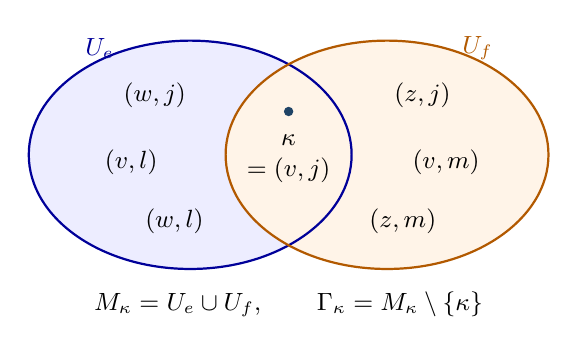
\begin{tikzpicture}[font=\small]
  \fill[blue!7] (-1.25,0) ellipse (2.05 and 1.45);
  \fill[orange!9] (1.25,0) ellipse (2.05 and 1.45);
  \draw[blue!60!black,thick] (-1.25,0) ellipse (2.05 and 1.45);
  \draw[orange!70!black,thick] (1.25,0) ellipse (2.05 and 1.45);
  \node[blue!60!black] at (-2.4,1.35) {$U_e$};
  \node[orange!70!black] at (2.4,1.35) {$U_f$};
  \node at (-1.7,.75) {$(w,j)$};
  \node at (-2.0,-.1) {$(v,l)$};
  \node at (-1.45,-.85) {$(w,l)$};
  \node at (1.7,.75) {$(z,j)$};
  \node at (2.0,-.1) {$(v,m)$};
  \node at (1.45,-.85) {$(z,m)$};
  \fill[linkblue] (0,.55) circle (1.7pt);
  \node[align=center] at (0,-.05) {$\kappa$\\$=(v,j)$};
  \node at (0,-1.9) {$M_\kappa=U_e\cup U_f,\qquad
                    \Gamma_\kappa=M_\kappa\setminus\{\kappa\}$};
\end{tikzpicture}
\caption{The seven coordinates available at the corner
$\kappa=(v,j)$, where $j=\{v,w,z\}$, $e=\{v,w\}$ and
$f=\{v,z\}$. The opposite faces on $e$ and $f$ are $l$ and $m$.
The two activation branches keep the same six outer coordinates;
one also keeps the common corner marked by the dot.}
\label{fig:kernel-corner-activation}
\end{figure}


Fix $0<\theta<1$. Give each corner a sign $\sigma_\kappa$, choosing
exactly one negative sign, for example $\sigma_{(0,0)}=-1$ and all
others $+1$. At the type pair $\kappa=(v,j)$ with $v\in j$ use this
\emph{base law}:
\begin{itemize}
\item with probability $1/2$, set $S=M_\kappa$ and give each sign
vector on $S$ probability
$2^{-7}(1+\sigma_\kappa\theta\prod_{\gamma\in\Gamma_\kappa}\xi_\gamma)$;
\item with probability $1/2$, set $S=\Gamma_\kappa$ and give each
sign vector on $S$ probability
$2^{-6}(1-\sigma_\kappa\theta\prod_{\gamma\in\Gamma_\kappa}\xi_\gamma)$.
\end{itemize}
These conditional masses are positive and sum to one because a
nonempty sign monomial has zero average under uniform signs. At a
nonincident type pair $(v,j)$ use $S=\varnothing$ deterministically.
Write $A^{\mathrm{base}}$ for the resulting moments.

Under either branch at a corner, the only nonempty sign monomial with
possibly nonzero expectation has index $\Gamma_\kappa$. Its conditional
expectations are respectively $\sigma_\kappa\theta$ and
$-\sigma_\kappa\theta$. The two effects of the branch choice are
\begin{equation}
 \E\phi_{\Gamma_\kappa}
 =\tfrac12\sigma_\kappa\theta-\tfrac12\sigma_\kappa\theta=0,
 \qquad
 A^{\mathrm{base}}_\kappa(U_e,U_f)
 =\tfrac12\sigma_\kappa\theta.
 \label{eq:kernel-branch-biases}
\end{equation}
The second identity holds because only the \(M_\kappa\) branch
contains \(U_e\cup U_f\), while their sign product is the
\(\Gamma_\kappa\) monomial. All base laws satisfy
Equation~\eqref{eq:kernel-zero-moments}, but this overlap moment can
have either sign.
More explicitly, for $Q=\alpha\cup\beta$ and
$R=\alpha\mathbin\triangle\beta$,
\begin{align}
 A^{\mathrm{base}}_\kappa(\alpha,\beta)
 &=\tfrac12\1_{\{Q\subseteq M_\kappa\}}
       \bigl(\1_{\{R=\varnothing\}}
                +\sigma_\kappa\theta\1_{\{R=\Gamma_\kappa\}}\bigr)
 \notag\\
 &\quad+\tfrac12\1_{\{Q\subseteq\Gamma_\kappa\}}
       \bigl(\1_{\{R=\varnothing\}}
                -\sigma_\kappa\theta\1_{\{R=\Gamma_\kappa\}}\bigr).
 \label{eq:kernel-base-moment}
\end{align}

\begin{lemma}[Support forcing]
\label{lem:kernel-support}
At the identity type assignments $a(i)=i$, $b(j)=j$, the sum in
Equation~\eqref{eq:kernel-coefficient} for the base laws has exactly one
nonzero term. Its labels and value are
\begin{equation}
 \alpha_e=U_e\quad(e\in E),\qquad
 C_{A^{\mathrm{base}}}(\mathrm{id},\mathrm{id})
 =-(\theta/2)^{66}.
 \label{eq:kernel-negative-term}
\end{equation}
\end{lemma}

\begin{proof}
We first prove the support identity
\begin{equation}
 \bigcap_{\kappa\in U_g}M_\kappa=U_g
 \qquad(g\in E).
 \label{eq:kernel-support-intersection}
\end{equation}
The same set \(\mathscr C\) indexes coordinates \(\gamma\) and
activation corners \(\kappa\). Availability is symmetric:
\(\gamma\in M_\kappa\) if and only if \(\kappa\in M_\gamma\).
Both conditions mean that the two corners lie in a common set \(U_e\).
Fix a coordinate $\gamma=(v,j)$, write $j=\{v,w,z\}$, and let
$e=\{v,w\}$, $f=\{v,z\}$ have opposite faces $l,m$, respectively.
This coordinate belongs to precisely $U_e$ and $U_f$. Consequently it
is available at exactly the following activation corners: all three
corners of $j$, the two $e$-endpoint corners of $l$, and the two
$f$-endpoint corners of $m$. To be available at all four corners of
$g$, its two faces must therefore be among $j,l,m$. The choice $j,l$
forces $g=e$, and $j,m$ forces $g=f$, since distinct triples share at
most one pair. The choice $l,m$ cannot work: its two endpoints would
both have to lie in $\{v,w\}\cap\{v,z\}=\{v\}$. Thus the coordinate
$\gamma$ is available at every corner of $g$ if and only if
$g\in\{e,f\}$, equivalently if and only if $\gamma\in U_g$.
This proves Equation~\eqref{eq:kernel-support-intersection}.

In a nonzero identity-type term, $\alpha_g$ must lie in the maximal
activation support at each of the four corners of $g$. Hence
$\alpha_g\subseteq U_g$. At a corner $\kappa$ with pairs $e,f$, the
two nonempty labels cannot be disjoint by
Equation~\eqref{eq:kernel-disjoint-zero}. Since
$U_e\cap U_f=\{\kappa\}$, both labels contain $\kappa$. Applying
this at all four corners of $g$ gives $\alpha_g=U_g$.

For these labels, Equation~\eqref{eq:kernel-branch-biases} gives
the local factor \(\sigma_\kappa\theta/2\). Multiplying the $66$ factors,
with exactly one negative $\sigma_\kappa$, proves the assertion.
\end{proof}

Each local matrix $A^{\mathrm{base}}_\kappa$ is positive semidefinite,
being a matrix of second moments of the random variables $\phi_\alpha$.
For example its principal block on $U_e,U_f$ is
\[
 \begin{pmatrix}1/2&\sigma_\kappa\theta/2\\
                 \sigma_\kappa\theta/2&1/2\end{pmatrix},
\]
with eigenvalues $(1+\theta)/2$ and $(1-\theta)/2$. Thus the negative
global term uses an admissible negative off-diagonal moment. The
support argument proves that local diagonal alternatives cannot form
any additional nonempty global labeling at the identity types.

\subsection{Pinning the types by color refinement}

The identity calculation alone does not control the kernel density:
the expansion averages over every type assignment, including maps with
repetitions. We now give the identity strictly larger score than every
competitor. The following lemma applies to any bipartite graph whose
part colors refine to distinct vertex colors.

\begin{lemma}[Pinning by vertex and pair scores]
\label{lem:pinning}
Let $F=(P\sqcup Q,L)$ be a finite bipartite graph for which color
refinement, starting with the two part colors, becomes discrete within
each part. There are real vertex scores $s_t$, $t\in P\sqcup Q$,
and pair scores $s_{ab}$, $(a,b)\in P\times Q$, such that the identity
is the unique maximizer of
\begin{equation}
 \mathcal Q(f)=\sum_{u\in P\sqcup Q}s_{f(u)}
              +\sum_{\{u,v\}\in L,\ u\in P}s_{f(u)f(v)}
 \label{eq:kernel-pinning-score}
\end{equation}
over \emph{all} maps $f$ preserving the two parts. In particular the
maximum has a positive gap from every other such map; no injectivity
or adjacency-preservation condition is imposed.
\end{lemma}

\begin{proof}
Let $\ell_0$ be the two part colors and, at round $t$, let $h_t(u)$
be the histogram of $\ell_{t-1}$-colors among the neighbors of $u$.
The new color is $\ell_t(u)=(\ell_{t-1}(u),h_t(u))$. Choose $R\ge1$
rounds giving a discrete coloring. At round $t$ assign the vertex score
$-\|h_t(a)\|^2$ to type $a$ and the pair score
\[
 2h_t(a)(\ell_{t-1}(b))+2h_t(b)(\ell_{t-1}(a))
\]
to every $(a,b)\in P\times Q$, including nonedges. The total round
score of \(f\) is
\[
 F_t(f)=-\sum_u\|h_t(f(u))\|^2
 +2\sum_u\sum_{v\in N_F(u)}
     h_t(f(u))\bigl(\ell_{t-1}(f(v))\bigr).
\]
Here \(N_F(u)\) is the neighbor set of \(u\). Both sums are indexed
by the vertices and directed incidences of the source graph \(F\),
even when \(f\) repeats a type.

If $\ell_{t-1}(f(u))=\ell_{t-1}(u)$ for every $u$, the inner
neighbor sum equals $\langle h_t(f(u)),h_t(u)\rangle$. Thus
\begin{align}
 F_t(f)
 &=\sum_u\bigl(2\langle h_t(f(u)),h_t(u)\rangle
                   -\|h_t(f(u))\|^2\bigr)\notag\\
 &=\sum_u\|h_t(u)\|^2
       -\sum_u\|h_t(f(u))-h_t(u)\|^2.
 \label{eq:kernel-pinning-square}
\end{align}
The first equality uses only preservation of previous colors. It
therefore applies to noninjective maps and to maps taking edges to
nonedges. In this situation $F_t(\mathrm{id})-F_t(f)$ is a nonnegative
integer, zero precisely when $f$ also preserves all new colors.

To combine the rounds into a single score, set
\[
 M=\max_{f,\,1\le t\le R}|F_t(f)-F_t(\mathrm{id})|,
 \qquad L_0=M+2,
 \qquad \mathcal Q(f)=\sum_{t=1}^R L_0^{R-t}F_t(f).
\]
The maximum defining $M$ is finite. For a nonidentity map, let $t$
be the first round at which a color fails to be preserved. All
earlier scores tie the identity; the loss at round $t$ is at least
$L_0^{R-t}$. Its possible later advantage is at most
\[
 M\sum_{j=0}^{R-t-1}L_0^j<L_0^{R-t}.
\]
Hence its total score is strictly smaller. A nonidentity map must
have such a first round because the final colors are discrete.
The weighted sums of the round vertex scores and pair scores are the
required $s_t,s_{ab}$. Finiteness of the set of maps gives the positive
gap.
\end{proof}

Apply Lemma~\ref{lem:pinning} to $H$, using
Proposition~\ref{prop:complex}. Let its scores be $s_a$ on $I$, $s_b$
on $J$, and $s_{ab}$ on $I\times J$. For a positive parameter $\rho$,
choose priors and thinning probabilities
\begin{equation}
 \pi_a=\frac{e^{\rho s_a}}{Z_I},\qquad
 \nu_b=\frac{e^{\rho s_b}}{Z_J},\qquad
 \lambda_{ab}=e^{\rho(s_{ab}-s_{\max})},\qquad
 s_{\max}=\max_{a,b}s_{ab},
 \label{eq:kernel-priors}
\end{equation}
where $Z_I=\sum_{a\in I}e^{\rho s_a}$ and
$Z_J=\sum_{b\in J}e^{\rho s_b}$. Since $0<\lambda_{ab}\le1$, the
following is a probability law: use the entire base law with
probability $\lambda_{ab}$, and use $S=\varnothing$ otherwise.
Its moments satisfy the exact identity
\begin{equation}
 A^\lambda_{ab}(\alpha,\beta)
 =\lambda_{ab}A^{\mathrm{base}}_{ab}(\alpha,\beta)
 +(1-\lambda_{ab})\1_{\{\alpha=\beta=\varnothing\}}.
 \label{eq:kernel-thinning}
\end{equation}
This preserves Equation~\eqref{eq:kernel-zero-moments}. In every
all-nonempty term it introduces one factor $\lambda_{ab}$ per
incidence, independently of the sizes of the coordinate subsets.

Let $C(a,b)=C_{A^{\mathrm{base}}}(a,b)$ and let $t_0$ be the
coefficient of the nonempty terms in
Equation~\eqref{eq:kernel-expansion} for the thinned laws and these
priors. By Equation~\eqref{eq:kernel-thinning},
\begin{align}
 t_0
 &=Z_I^{-13}Z_J^{-22}e^{-66\rho s_{\max}}
     \sum_{a:I\to I\,,\ b:J\to J}
           C(a,b)e^{\rho\mathcal Q(a,b)}.
 \label{eq:kernel-pinned-coefficient}
\end{align}
All normalizing factors outside the sum are common to every map.
Here $\mathcal Q(a,b)$ means the score of the part-preserving map
specified by $a,b$.

Write $Q_*=\mathcal Q(\mathrm{id},\mathrm{id})$, and let
\[
 \delta_*=\min_{(a,b)\ne(\mathrm{id},\mathrm{id})}
          (Q_*-\mathcal Q(a,b))>0,
 \qquad
 B_*=\sum_{(a,b)\ne(\mathrm{id},\mathrm{id})}|C(a,b)|<\infty.
\]
After division by $e^{\rho Q_*}$, the absolute value of the
competitor sum is at most $B_*e^{-\rho\delta_*}$. Choose a fixed
finite $\rho>0$ large enough that
\begin{equation}
 B_*e^{-\rho\delta_*}<(\theta/2)^{66};
 \label{eq:kernel-finite-gap}
\end{equation}
if $B_*=0$, any positive $\rho$ suffices. By
Equation~\eqref{eq:kernel-negative-term} this makes $t_0<0$.

\subsection{Dilution, symmetrization, and finite hosts}

We have made the limiting nonempty coefficient negative in one
orientation. The symmetric kernel below multiplies the densities in
both orientations. Dilution makes the negative term dominate the
unknown term from the other orientation.

Keep $\theta,\rho$, the priors, and all the thinned laws fixed. Add
an inactive type $*$ to $\mathcal A=I$, giving it probability
$1-\varepsilon$ and giving each old type $a$ probability
$\varepsilon\pi_a$, where $0<\varepsilon<1$. Every pair involving
$*$ uses $S=\varnothing$. Keep the $J$-type prior $\nu$ unchanged.
Let $W_{q,\varepsilon}$ be the resulting kernel.

For precision, define also the finite coefficient for the opposite
orientation before dilution:
\begin{align}
 t_1={}&\sum_{b:I\to J\,,\ a:J\to I}
       \left(\prod_{i\in I}\nu_{b(i)}\right)
       \left(\prod_{j\in J}\pi_{a(j)}\right)
       \sum_{\substack{\alpha_e\subseteq\mathscr C\ (e\in E)\\
                       \alpha_e\ne\varnothing\ (e\in E)}}
       \prod_{(i,j)\in\mathscr C}
       A^\lambda_{a(j)b(i)}
         \bigl(\alpha_{e(i,j)},\alpha_{f(i,j)}\bigr).
 \label{eq:kernel-transpose-coefficient}
\end{align}
Both $t_0<0$ and $t_1\in\R$ are independent of $q$ and
$\varepsilon$.

In a nonempty-label term, a vertex with inactive type gives a zero
factor on each of its incidences. Every vertex of $H$ has positive
degree, so every original $I$-type draw must be active. There are
$13$ such draws for $W_{q,\varepsilon}$ and $22$ for its transpose.
Lemma~\ref{lem:kernel-expansion} therefore gives the exact limiting
coefficients
\begin{align}
 t_{I,J}(W_{q,\varepsilon})
   &=1+\varepsilon^{13}t_0+o(1),\notag\\
 t_{I,J}(W_{q,\varepsilon}^\top)
   &=1+\varepsilon^{22}t_1+o(1).
 \label{eq:kernel-dilution}
\end{align}
These errors tend to zero with $q$ after $\varepsilon$ is fixed.
In particular, the limiting product is
\begin{equation}
 (1+\varepsilon^{13}t_0)(1+\varepsilon^{22}t_1)
 =1+\varepsilon^{13}
      \bigl(t_0+\varepsilon^9t_1+\varepsilon^{22}t_0t_1\bigr)<1
 \label{eq:kernel-product-gap}
\end{equation}
for all sufficiently small positive $\varepsilon$, because the
bracket tends to $t_0<0$. Choose one such $\varepsilon$ and then a
sufficiently large odd prime $q$. The cancellation of $c_0$ in the
coordinate expansion makes the limiting coefficients independent of
the congruence class of $q$. The resulting fixed kernel $W$ is
nonnegative, finite, has mean one, and satisfies
\begin{equation}
 t_{I,J}(W)t_{I,J}(W^\top)<1.
 \label{eq:kernel-oriented-gap}
\end{equation}

\begin{proposition}
\label{prop:negative-kernel}
Assuming Lemma~\ref{lem:rank-layer}, there is a symmetric kernel
$U:\Omega\times\Omega\to[0,1]$ on a finite probability space with
mean $\mu>0$ such that
\begin{equation}
 t(H,U)<\mu^{66}.
 \label{eq:kernel-symmetric-gap}
\end{equation}
\end{proposition}

\begin{proof}
Use the kernel $W:\mathcal X\times\mathcal Y\to[0,\infty)$ just
constructed and set $\Omega=\mathcal X\times\mathcal Y$ with product
probability. Define
\begin{equation}
 V\bigl((x,y),(x',y')\bigr)=W(x,y')W(x',y).
 \label{eq:kernel-crossed-product}
\end{equation}
This kernel is symmetric, nonnegative, and has mean one: the two
factors on the right use independent variables and each has mean
one. In its product over $H$, the factors using $x_i$ for $i\in I$
and $y_j$ for $j\in J$ are independent of those using $y_i$ for
$i\in I$ and $x_j$ for $j\in J$. Therefore
\[
 t(H,V)=t_{I,J}(W)t_{I,J}(W^\top)<1.
\]
Let $L=\max V$, which is finite and at least one, and set $U=V/L$.
Then $0\le U\le1$, $\mu=\E U=1/L>0$, and homogeneity gives
$t(H,U)=L^{-66}t(H,V)<L^{-66}=\mu^{66}$.
\end{proof}

We use the standard independent sampling construction for graphons
\cite[Section~2.6, Lemma~2.4]{lovaszszegedy2006}. The following argument keeps the collision
error explicit and counts all homomorphisms.

\begin{lemma}[Transfer to a finite simple host]
\label{lem:finite-host}
Suppose $U$ is a symmetric $[0,1]$-valued kernel on a finite
probability space, $\mu=\E U>0$, and
\[
 \tau=t(H,U),\qquad \Delta=\mu^{66}-\tau>0.
\]
For any integer
\begin{equation}
 n>\frac{595+66\mu^{66}}{\Delta},
 \label{eq:kernel-host-size}
\end{equation}
there is a finite simple graph $G$ on $n$ vertices with
$t(H,G)<p(G)^{66}$.
\end{lemma}

\begin{proof}
Sample labels $z_1,\ldots,z_n$ independently from the probability
space of $U$. Conditional on these labels, put an edge on each
unordered pair of distinct vertices $\{a,b\}$ independently with
probability $U(z_a,z_b)$. No loops are drawn. This defines a random
finite simple undirected graph $G_n$, and
\begin{equation}
 \E p(G_n)=(1-1/n)\mu.
 \label{eq:kernel-host-mean}
\end{equation}

For every injective map $f:V(H)\to\{1,\ldots,n\}$, its image
vertices have independent labels, and its $66$ source edges use
distinct unordered host pairs. Its probability of being a
homomorphism is exactly $\tau$. Among all $n^{35}$ maps, the
proportion that identify any two source vertices is at most
$\binom{35}{2}/n=595/n$, by the union bound. Each such map has a
homomorphism indicator between zero and one; a collision on a
source edge gives zero, while any repeated host edges are counted
by their actual single Bernoulli trials. No independence claim for
these maps is needed. Comparing their contribution with $\tau$
times their proportion gives
\begin{equation}
 |\E t(H,G_n)-\tau|\le\frac{595}{n}.
 \label{eq:kernel-collision-bound}
\end{equation}
Thus the density still counts all homomorphisms, including every
noninjective one.

Using $(1-1/n)^{66}\ge1-66/n$, Equations~\eqref{eq:kernel-host-size}
and~\eqref{eq:kernel-collision-bound} give
\begin{align*}
 \E t(H,G_n)
 &\le\mu^{66}-\Delta+595/n\\
 &<\mu^{66}-66\mu^{66}/n\\
 &\le\bigl((1-1/n)\mu\bigr)^{66}
   =\bigl(\E p(G_n)\bigr)^{66}
   \le\E\bigl[p(G_n)^{66}\bigr].
\end{align*}
The last inequality is convexity. Hence some realization has
$t(H,G_n)<p(G_n)^{66}$. Such a realization cannot be edgeless.
\end{proof}

Proposition~\ref{prop:negative-kernel} and Lemma~\ref{lem:finite-host}
prove Theorem~\ref{thm:main} conditional only on
Lemma~\ref{lem:rank-layer}. To summarize the order of choices, fix a
sufficiently large even $D$, the $66$ coordinates and $\theta$, then
the scores and a finite $\rho$ satisfying Equation~\eqref{eq:kernel-finite-gap},
then a positive $\varepsilon$ satisfying
Equation~\eqref{eq:kernel-product-gap}, and then a sufficiently large
odd prime $q$. Only after fixing and scaling this finite kernel are
$\mu,\Delta$ and the host size $n$ chosen.
Sections~\ref{sec:transverse}--\ref{sec:tail} establish the required
rank-layer limit.

\section{Transverse configurations and determinant signs}
\label{sec:transverse}

We begin the proof of Lemma~\ref{lem:rank-layer} with the configurations
whose point differences are nonsingular. Throughout this section $D=2r$
is fixed, $q$ tends to infinity through odd primes, and constants in
$O(\cdot)$ may depend on $D$. We use $b(n)=n(n+1)/2$, including $b(0)=0$.
The estimates concerning growing $D$ will be made separately in
Section~\ref{sec:tail}.

On triples with nonsingular point differences, for two or three active
incidences on a face, the sign model has value
\(2\) or \(8\) when every active pair satisfies
\(\chi(\det(X_i-X_k))=c_0\xi_{ij}\xi_{kj}\), and value \(0\) when a
match fails. For \(r>1\), we will approximate the normalized center
factor by this model in \(L^1\) on these triples, and bound that
factor uniformly there. These estimates
permit multiplication over faces sharing point matrices. The
preliminary counts fix the layer normalizations and enumerate the
candidate subspaces; restriction-sign balance supplies the final
factor \(1/2\). We then prove that the determinant signs on all
\(33\) point pairs have an asymptotically independent joint law.

\subsection{Symmetric forms over a finite field}

The discriminant sign of a symmetric form is the quadratic character of
the determinant of its induced nondegenerate form on the quotient by
its radical. A change of basis multiplies this determinant by a square,
so its character is well defined. In dimension zero the determinant is
understood to be $1$.

Rank and discriminant sign are the standard invariants of symmetric
bilinear forms over a finite field of odd order. Exact counts by these
invariants appear, for example, in
Schmidt~\cite[Section~2, Proposition~2.1]{schmidt2015}.
We give the elementary estimates needed here, with their proofs.

\begin{lemma}[Subspaces and symmetric matrices]
\label{lem:symmetric-counts}
For $0\leq k\leq n$, the number of $k$-dimensional subspaces of
$\F_q^n$ is
\begin{equation}
\label{eq:transverse-grassmann}
 \genfrac{[}{]}{0pt}{}{n}{k}_q
 =\prod_{a=0}^{k-1}\frac{q^n-q^a}{q^k-q^a}
 =q^{k(n-k)}(1+O(q^{-1})).
\end{equation}
For a uniform matrix $M\in\mathcal S_n$, with $n\geq 1$,
\[
 \P(M\text{ is nonsingular})=1-O(q^{-1}),\qquad
 \P(\chi(\det M)=\xi)=\frac12+O(q^{-1})
 \quad(\xi\in\{+1,-1\}).
\]
For $1\leq k\leq n$, the probability of rank $k$ and prescribed
discriminant sign is
\begin{equation}
\label{eq:transverse-signed-rank}
 \left(\frac12+O(q^{-1})\right)q^{-b(n-k)}.
\end{equation}
Finally, for $0\leq u\leq n$,
\begin{equation}
\label{eq:transverse-nullity}
 \P(\dim\ker M\geq u)=O(q^{-b(u)}).
\end{equation}
\end{lemma}

\begin{proof}
Count ordered linearly independent $k$-tuples in $\F_q^n$ and divide
by the number of ordered bases of $\F_q^k$ to obtain
Equation~\eqref{eq:transverse-grassmann}. Its asymptotic follows by factoring
out the displayed powers of $q$; all products have fixed length.

For the nonsingularity and sign assertions, use induction on $n$.
On the event that the leading $(n-1)$-dimensional principal minor $C$
is nonsingular, write
\[
 M=\begin{pmatrix}C&z\\z^{\mathsf T}&a\end{pmatrix},\qquad
 \det M=\det C\,(a-z^{\mathsf T}C^{-1}z).
\]
Given $C,z$, the final scalar factor is uniform on $\F_q$. It is zero
with probability $q^{-1}$ and has either nonzero character with
probability $(q-1)/(2q)$. The exceptional principal minor has probability
$O(q^{-1})$ by induction. The same argument starts at $n=1$ with the
empty principal minor.

For the rank assertion, fix a $k$-subspace $U$ with basis-column matrix
$P$. Every symmetric matrix with image $U$ is uniquely
$PRP^{\mathsf T}$ for a nonsingular symmetric $k$-by-$k$ matrix $R$.
Indeed, if $Q P$ is the identity, symmetry and the image condition give
$M=P(QMQ^{\mathsf T})P^{\mathsf T}$, and multiplication by $Q,Q^{\mathsf T}$
also proves uniqueness. The surjection $P^{\mathsf T}:\F_q^n\to\F_q^k$
identifies the nondegenerate quotient form with $R$, so the discriminant
sign is $\chi(\det R)$. Consequently the desired count is
\[
 \genfrac{[}{]}{0pt}{}{n}{k}_q\,q^{b(k)}
 \left(\frac12+O(q^{-1})\right).
\]
Divide by $q^{b(n)}$ and use
$k(n-k)+b(k)-b(n)=-b(n-k)$.

For Equation~\eqref{eq:transverse-nullity}, sum over $u$-subspaces $U$
contained in the radical. In a basis beginning with $U$, this containment
sets to zero the first $u$ rows and columns, imposing
$nu-\binom u2$ independent linear conditions. A uniform symmetric form
therefore has $U$ in its radical with probability
$q^{-nu+\binom u2}$. Multiplication by
$\genfrac{[}{]}{0pt}{}{n}{u}_q=O(q^{u(n-u)})$ gives the assertion.
\end{proof}

In particular, writing $\pi_\xi$ for the mass of the signed rank-$r$
layer in $\mathcal S_D$, we have
\begin{equation}
\label{eq:transverse-signed-mass}
 \pi_\xi=\left(\frac12+O(q^{-1})\right)q^{-b(r)},
 \qquad \pi_\xi^{-1}=2q^{b(r)}(1+O(q^{-1})).
\end{equation}
These are the normalizations in $K_\xi$.

A subspace is \emph{totally isotropic} for a symmetric bilinear form
if the form vanishes on every pair of vectors in that subspace.
The next count is the split orthogonal counterpart of the symplectic
counts in Section~\ref{sec:orbits}; see also Taylor~\cite[Exercise~11.3]{taylor1992}.

\begin{lemma}[Split forms and their maximal isotropic subspaces]
\label{lem:transverse-split}
Let $r\geq1$. A nondegenerate symmetric form on a $2r$-dimensional
space over $\F_q$
has an $r$-dimensional totally isotropic subspace if and only if its
determinant character is $c_0=\chi((-1)^r)$. Such a form is a direct
orthogonal sum of $r$ hyperbolic planes. The total number of its
$r$-dimensional totally isotropic subspaces is
\begin{equation}
\label{eq:transverse-isotropic-count}
 N_r=\prod_{a=0}^{r-1}(1+q^a)
 =2q^{r(r-1)/2}(1+O(q^{-1})).
\end{equation}
The count includes both families of maximal isotropic subspaces.
\end{lemma}

\begin{proof}
First, a nondegenerate symmetric form has an orthogonal basis. A
nonzero form has a vector of nonzero norm, since otherwise polarization
would make the form zero. Split off this nondegenerate line and continue
on its orthogonal complement.

For any $a,b\in\F_q^\times$ and $t\in\F_q$, the two sets
$\{ax^2:x\in\F_q\}$ and $\{t-by^2:y\in\F_q\}$ each have size
$(q+1)/2$ and therefore meet. Thus $ax^2+by^2=t$ is solvable. A diagonal
nondegenerate form in at least three variables consequently has a
nonzero isotropic vector: solve $ax^2+by^2=-c$ and set the third
coordinate to $1$. Given an isotropic vector $e\ne0$, choose $f$ with
$\langle e,f\rangle=1$ and replace $f$ by
$f-\langle f,f\rangle e/2$. The resulting plane has Gram matrix
$\left(\begin{smallmatrix}0&1\\1&0\end{smallmatrix}\right)$ and splits
off orthogonally. Repetition leaves an anisotropic space of dimension
at most two. In dimension two, $ax^2+by^2$ is isotropic exactly when
$\chi(-ab)=1$, or equivalently when its determinant character is
$\chi(-1)$. Each hyperbolic plane also has determinant character
$\chi(-1)$. This proves that the determinant condition is precisely
the condition that the entire $2r$-space split into hyperbolic planes.

A split form has the required isotropic subspace, spanned by one vector
from each hyperbolic pair. Conversely, if such a subspace $U$ is given,
split off a hyperbolic plane using $e\in U$. Its orthogonal complement
has an isotropic $(r-1)$-subspace: for $u\in U$, replace $u$ by
$u-\langle u,f\rangle e$. This linear map on $U$ has kernel
$\langle e\rangle$, so its image has dimension $r-1$.
Induction shows that the entire form is split.

In split coordinates $(x,y)\in\F_q^r\oplus\F_q^r$, isotropy is the
equation $x^{\mathsf T}y=0$. There are
\[
 (q^r-1)q^{r-1}+(q^r-1)
 =(q^r-1)(q^{r-1}+1)
\]
nonzero isotropic vectors. The quotient $\ell^\perp/\ell$ by an
isotropic line has dimension $2r-2$. Splitting off a hyperbolic plane
through $\ell$ identifies this quotient with its nondegenerate
orthogonal complement, whose determinant character is
$\chi((-1)^{r-1})$. The criterion just proved makes the quotient split.
Count pairs $(\ell,U)$ with
$\ell\subset U$ and $\dim U=r$ to get
\[
 N_r\frac{q^r-1}{q-1}
 =\frac{(q^r-1)(q^{r-1}+1)}{q-1}N_{r-1}.
\]
With $N_0=1$, this gives the product in
Equation~\eqref{eq:transverse-isotropic-count}. In particular $N_1=2$;
no choice of one isotropic family has been imposed in this count.
\end{proof}

The isotropic-subspace count does not yet determine the sign of a
second form on those subspaces. The following averaged estimate
supplies that sign information for any sufficiently large family.

\begin{lemma}[Concentration of restriction signs]
\label{lem:transverse-restrictions}
Let $\mathcal U$ be any nonempty family of distinct $r$-subspaces of
$\F_q^D$, with $r\geq1$, and let $Q$ be a uniform symmetric form.
For $\xi\in\{+1,-1\}$ put
\[
 f_\xi(Q)=\frac1{|\mathcal U|}\sum_{U\in\mathcal U}
 \1_{\{Q|_U\text{ nonsingular of sign }\xi\}}.
\]
Uniformly over the family $\mathcal U$,
\begin{equation}
\label{eq:transverse-restriction-error}
 \E\left|f_\xi(Q)-\frac12\right|
 =O\left(q^{-1/2}+|\mathcal U|^{-1/2}\right).
\end{equation}
The same bound holds after conditioning $Q$ to be nonsingular, or
conditioning both $Q$ and $Q-L$ to be nonsingular, uniformly over every
fixed symmetric form $L$.
\end{lemma}

\begin{proof}
Restriction onto a fixed subspace is a surjective linear map on spaces
of symmetric forms, so each summand has expectation
$1/2+O(q^{-1})$ by Lemma~\ref{lem:symmetric-counts}.
For distinct $U,V\in\mathcal U$ write $T=U\cap V$. Extend a basis of
$T$ separately to bases of $U$ and $V$, and then to an ambient basis.
In this basis, the coefficients defining the two restricted forms
overlap exactly in the symmetric block on $T$. Thus any two forms on
$U,V$ agreeing on $T$ extend simultaneously to the ambient space;
given $Q|_T$, their remaining coefficients are independent and uniform.

If $T$ has positive dimension, its restriction is nonsingular outside
an event of probability $O(q^{-1})$; for $T=0$ this holds with probability
one. Given a nonsingular restriction on $T$, the determinant on $U$
is the determinant on $T$ times that of a uniform symmetric Schur
complement of size $r-\dim T>0$. The corresponding Schur complement
on $V$ is independent. Both signs are balanced up to $O(q^{-1})$,
uniformly over the fixed common block and mixed coefficients. The
covariance of the two indicator summands is therefore $O(q^{-1})$.
The diagonal covariance is at most $1$, giving
\[
 \Var(f_\xi)=O(q^{-1}+|\mathcal U|^{-1}).
\]
Cauchy--Schwarz and the expectation estimate prove
Equation~\eqref{eq:transverse-restriction-error}.

For the last assertion, each of $Q$ and $Q-L$ is marginally uniform.
The event $\mathcal A$ that the specified forms are nonsingular has
probability $1-O(q^{-1})$, uniformly in $L$. Since the error being
averaged is nonnegative,
\[
 \E\left[\left|f_\xi-\frac12\right|\,\middle|\,\mathcal A\right]
 \leq \frac{\E|f_\xi-1/2|}{\P(\mathcal A)}.
\]
This proves the same bound under either conditioning.
\end{proof}

\subsection{Counting centers on one face}

The following projection identity explains the special role of half
rank.

\begin{lemma}[Complementary images]
\label{lem:transverse-projection}
Suppose $B\in\mathcal S_{2r}$ is nonsingular and $A\in\mathcal S_{2r}$
has rank $r$. Then
\begin{equation}
\label{eq:transverse-projection}
 \rank(B-A)=r\quad\Longleftrightarrow\quad AB^{-1}A=A.
\end{equation}
If $A$ and $A-B$ have discriminant signs $\xi_1,\xi_2$, respectively,
under these conditions, then
\begin{equation}
\label{eq:transverse-pair-sign}
 \chi(\det B)=c_0\xi_1\xi_2.
\end{equation}
\end{lemma}

\begin{proof}
If $A$ and $B-A$ both have rank $r$, their images span the image of
$B$, so these images are complementary. Since
$AB^{-1}+(B-A)B^{-1}$ is the identity, uniqueness of the corresponding
direct-sum decomposition makes $AB^{-1}$ the projection onto the first
image. In particular $AB^{-1}A=A$. Conversely, this identity makes
$AB^{-1}$ an idempotent of rank $r$. Its complementary idempotent has
rank $r$ and, after multiplication by $B$, equals $B-A$.

Choose basis-column matrices $P_1,P_2$ of the two complementary images
and write $A=P_1R_1P_1^{\mathsf T}$ and
$A-B=P_2R_2P_2^{\mathsf T}$. Then
\[
 B=(P_1\ P_2)\diag(R_1,-R_2)(P_1\ P_2)^{\mathsf T}.
\]
Taking determinant characters gives
Equation~\eqref{eq:transverse-pair-sign}.
\end{proof}

For independent point matrices $(X_i)_{i\in I}$ define
\begin{equation}
\label{eq:transverse-event}
 \eta_e^X=\chi(\det(X_i-X_k))\quad(e=\{i,k\}),\qquad
 \mathcal T=\{X_i-X_k\text{ nonsingular for every }e\in E\}.
\end{equation}
The choice of orientation of $e$ is immaterial because $D$ is even.
Each difference is uniform in $\mathcal S_D$, so
$\P(\mathcal T^c)=O(q^{-1})$ by Lemma~\ref{lem:symmetric-counts}.
For an activity pattern $B\subseteq\mathscr C$, let
$A_j=\{i\in j:(i,j)\in B\}$ and define the local center factor and its
sign model by
\begin{align}
 F_j(X)&=\E_{Y_j}\prod_{i\in A_j}K_{\xi_{ij}}(X_i-Y_j),
 \label{eq:transverse-face-factor}\\
 G_j(X)&=\prod_{\{i,k\}\subseteq A_j}
       (1+c_0\eta^X_{\{i,k\}}\xi_{ij}\xi_{kj}).
 \label{eq:transverse-model}
\end{align}
On transverse local configurations, $G_j$ equals $2$ for two active
incidences whose pair signs match, and $8$ for three active incidences
whose three pair signs match; it is zero when any required match fails.
With at most one active incidence, both $F_j$ and $G_j$ equal $1$.

\begin{lemma}[Local transverse approximation]
\label{lem:local-transverse}
Suppose $r>1$. For each face $j$, let $\mathcal T_j$ be the event that
all three differences between its point matrices are nonsingular.
Then, uniformly over the activity and sign choices,
\begin{equation}
\label{eq:transverse-local-l1}
 \E\bigl[\1_{\mathcal T_j}|F_j-G_j|\bigr]=O(q^{-1/2}).
\end{equation}
Moreover $0\leq F_j\leq C_D$ on $\mathcal T_j$, for a constant $C_D$
independent of $q$, and $0\leq G_j\leq8$ everywhere.
\end{lemma}

\begin{proof}
First suppose all three incidences are active, and locally write their
point matrices as $X_1,X_2,X_3$ and their signs as $\xi_1,\xi_2,\xi_3$.
Set
\[
 B_0=X_1-X_2,\quad B_1=X_1-X_3,\quad A=X_1-Y,
 \qquad Q=B_0^{-1},\quad L=B_0^{-1}-B_1^{-1}.
\]
On $\mathcal T_j$, the form
$L=B_0^{-1}(B_1-B_0)B_1^{-1}$ is symmetric and nonsingular. Write a
rank-$r$ matrix $A$ as $PRP^{\mathsf T}$. By
Lemma~\ref{lem:transverse-projection}, its other two rank conditions are
equivalent to
\[
 R(P^{\mathsf T}B_\nu^{-1}P)R=R\quad(\nu=0,1),
\]
or to
\begin{equation}
\label{eq:transverse-center-parametrization}
 P^{\mathsf T}LP=0,\qquad
 P^{\mathsf T}QP\text{ nonsingular},\qquad
 R=(P^{\mathsf T}QP)^{-1}.
\end{equation}
Thus the centers satisfying the three rank conditions are in bijection
with the maximal $L$-isotropic subspaces $U$ on which $Q$ restricts
nonsingularly. Changing the basis of $U$ leaves the resulting $A$
unchanged, and every $A$ recovers $U$ as its image, proving the stated
bijection.

Let $\mathcal M$ be the event that all three required pair matches
$\eta^X_{\{a,b\}}=c_0\xi_a\xi_b$ hold. If any match fails, the signed
count is zero by Equation~\eqref{eq:transverse-pair-sign}. If they all
hold, then
\[
 \chi(\det L)
 =\eta^X_{\{1,2\}}\eta^X_{\{1,3\}}\eta^X_{\{2,3\}}
 =c_0,
\]
so $L$ is split by Lemma~\ref{lem:transverse-split}. In
Equation~\eqref{eq:transverse-center-parametrization}, the sign of $A$
is the sign of $Q|_U$, since inversion preserves a nonzero determinant
character. Once it equals $\xi_1$, the pair matches with point $1$
force the other two signs to equal $\xi_2,\xi_3$.

For split $L$, let $f_{\xi_1}(Q;L)$ denote the fraction of its $N_r$
maximal isotropic subspaces having a nonsingular restriction of sign
$\xi_1$. On a matching transverse triple the exact normalized count is
\begin{equation}
\label{eq:transverse-three-normalization}
 F_j=\frac{q^{-b(D)}N_r}{\pi_{\xi_1}\pi_{\xi_2}\pi_{\xi_3}}
       f_{\xi_1}(Q;L)
     =(16+O(q^{-1}))f_{\xi_1}(Q;L).
\end{equation}
Here the exponent cancels because
$r(r-1)/2-b(2r)+3b(r)=0$. The factor $16$ combines the leading
factor $2$ in $N_r$ with the three signed-layer normalization factors
$2$; the restriction-sign fraction will supply a further factor $1/2$.

We specify the probability law used for that fraction. Before any
invertibility conditioning, $B_0,B_1$ are independent uniform symmetric
matrices: this follows by conditioning on $X_1$ and translating the
independent matrices $X_2,X_3$. After requiring $B_0,B_1$ to be
nonsingular, inversion preserves their independent uniform laws on
nonsingular symmetric matrices. Conditional also on a fixed value of
$L=B_0^{-1}-B_1^{-1}$, the matrix $Q$ is therefore uniform on
\[
 \{Q\in\mathcal S_D:Q\text{ and }Q-L\text{ are nonsingular}\}.
\]
Each admissible $Q$ corresponds to exactly one ordered inverse pair
$(Q,Q-L)$, which verifies the conditional uniformity directly.
Requiring $L$ to be nonsingular is exactly the remaining transverse
condition. Lemma~\ref{lem:transverse-restrictions}, uniformly for every
fixed nonsingular split $L$, now gives
\begin{equation}
\label{eq:transverse-matching-error}
 \E\left[\1_{\mathcal M}
       \left|f_{\xi_1}(Q;L)-\frac12\right|
       \,\middle|\,\mathcal T_j,L\right]
 \leq \E\left[\left|f_{\xi_1}(Q;L)-\frac12\right|
       \,\middle|\,\mathcal T_j,L\right]
 =O(q^{-1/2}).
\end{equation}
We used $r>1$, for which $N_r^{-1/2}=O(q^{-1/2})$.
The matching indicator is kept inside the expectation; no additional
conditioning on the matches is used. For nonsplit $L$, the matching
event is empty and both the signed count and its model vanish.
Equations~\eqref{eq:transverse-three-normalization}
and~\eqref{eq:transverse-matching-error} prove the local error estimate
with limiting value $8$ on matches. The same exact formula, with
$0\leq f_{\xi_1}\leq1$, gives a uniform bound on every transverse
triple, including the exceptional restrictions.

For two active incidences, relabel them $1,2$ and put $B=X_1-X_2$ and
$Q=B^{-1}$. The same projection argument now parametrizes centers by
all $r$-subspaces $U$ for which $Q|_U$ is nonsingular. On the pair match
$\chi(\det B)=c_0\xi_1\xi_2$, only the sign $\xi_1$ of this restriction
needs to be imposed; off the match the count is zero. If $f_{\xi_1}(Q)$
is the fraction among all $\genfrac{[}{]}{0pt}{}{2r}{r}_q$ subspaces,
the exact count on the match is
\begin{equation}
\label{eq:transverse-two-normalization}
 F_j=\frac{q^{-b(D)}\genfrac{[}{]}{0pt}{}{2r}{r}_q}
              {\pi_{\xi_1}\pi_{\xi_2}}
       f_{\xi_1}(Q)
     =(4+O(q^{-1}))f_{\xi_1}(Q).
\end{equation}
The exponent identity here is $r^2-b(2r)+2b(r)=0$. Conditional on $B$
being nonsingular, $Q$ is uniform nonsingular symmetric. Apply
Lemma~\ref{lem:transverse-restrictions} with this single conditioning
and keep the matching indicator inside the expectation as before.
This gives limiting value $2$, error $O(q^{-1/2})$, and a uniform
bound on the nonsingular-pair event. Restricting further to
$\mathcal T_j$ can only decrease the nonnegative error expectation.
The remaining cases follow from the mean-one normalization of each
$K_\xi$ and translation invariance.
\end{proof}

\subsection{Joint distribution of the pair signs}

The pairs share point matrices, so marginal balance of their signs does
not give their joint distribution. For each nonempty subset moment,
we first establish a high-probability event for the difference minors
at a selected incident vertex, then condition on all entries except
its off-diagonal row vector and transpose and average over that vector.
Table~\ref{tab:complex} shows that the degree of each
vertex in $(I,E)$ is at most $6$:
its degree there equals its number of incident faces, since each face
contains two pairs through that point and each pair occurs twice.

\begin{lemma}[Joint determinant signs]
\label{lem:joint-signs}
For fixed even $D\geq12$, the law of $(\eta_e^X)_{e\in E}$ converges
in total variation to that of independent uniform signs on
$\{+1,-1\}^E$.
\end{lemma}

\begin{proof}
Fix a nonempty subset $F\subseteq E$, and choose a vertex $i$ incident
with $s\geq1$ of its pairs. Write $N=D-1$ and, for every point $v$,
write its matrix in block form
\[
 X_v=\begin{pmatrix}a_v&z_v^{\mathsf T}\\z_v&W_v\end{pmatrix},
 \qquad W_v\in\mathcal S_N,\quad z_v\in\F_q^N.
\]
Let $k_1,\ldots,k_s$ be the selected neighbors of $i$, and put
$M_\ell=W_i-W_{k_\ell}$. We first establish a high-probability event
using these lower-right blocks, before conditioning on the other
entries. Given $W_i$, the $M_\ell$ are independent uniform symmetric
matrices. All are nonsingular except with probability $O(q^{-1})$.
Conditional on their nonsingularity, their inverses are independent
uniform nonsingular symmetric matrices.

Let $Q_1,\ldots,Q_s$ instead be independent uniform matrices in
$\mathcal S_N$. For any $t\in\F_q^s\setminus\{0\}$, the matrix
$\sum_\ell t_\ell Q_\ell$ is uniform in $\mathcal S_N$: condition on
all but a coordinate with nonzero coefficient. By
Equation~\eqref{eq:transverse-nullity}, its probability of rank at most
$s$ is $O(q^{-b(N-s)})$. The union bound over all nonzero $t$ gives
\[
 \P\left(\exists t\ne0:
       \rank\left(\sum_\ell t_\ell Q_\ell\right)\leq s\right)
 =O(q^{s-b(N-s)}).
\]
Conditioning all the $Q_\ell$ to be nonsingular divides this upper bound
by a probability $1-O(q^{-1})$. It follows that the event
\begin{equation}
\label{eq:transverse-good-minors}
 \mathcal G=\left\{\begin{array}{l}
 M_\ell\text{ is nonsingular for every }\ell,\\
 \rank(\sum_\ell t_\ell M_\ell^{-1})\geq s+1
       \text{ for every }t\in\F_q^s\setminus\{0\}
 \end{array}\right\}
\end{equation}
satisfies
\begin{equation}
\label{eq:transverse-good-probability}
 \P(\mathcal G^c)=O(q^{-1}+q^{s-b(N-s)})=O(q^{-1}).
\end{equation}
Indeed $s\leq6$ and $D\geq12$ imply $N-s\geq5$ and
$b(N-s)\geq15>s$. These probability bounds hold given every $W_i$
and hence hold without conditioning as well.

Only now condition on all entries of all point matrices except $z_i$.
The event $\mathcal G$ is determined by this conditioning, whereas
$z_i$ remains uniform on $\F_q^N$. On every such fixed configuration
in $\mathcal G$, the determinant formula gives
\begin{equation}
\label{eq:transverse-schur-evaluations}
 \det(X_i-X_{k_\ell})=\det(M_\ell)h_\ell(z_i),\qquad
 h_\ell(z)=a_i-a_{k_\ell}
 -(z-z_{k_\ell})^{\mathsf T}M_\ell^{-1}(z-z_{k_\ell}).
\end{equation}
Let $\mu$ be the law of $(h_1(z),\ldots,h_s(z))$ for uniform $z$.
Fix a nontrivial additive character $\psi$ of $\F_q$ and define
$\widehat\mu(t)=\E_z\psi(\sum_\ell t_\ell h_\ell(z))$.
The quadratic part at every frequency $t\ne0$ has rank at least $s+1$
by Equation~\eqref{eq:transverse-good-minors}.

We use the standard rank bound for a quadratic Gauss sum; see
Gowers and Wolf~\cite[Lemma~3.3]{gowerswolf2011}. The short differencing argument
also fixes our normalization. A quadratic polynomial
$p(z)=z^{\mathsf T}Hz+\lambda^{\mathsf T}z+c$ with symmetric quadratic
matrix $H$ obeys
\begin{align*}
 \left|\E_z\psi(p(z))\right|^2
 &=\E_{z,u}\psi(p(z+u)-p(z))\\
 &=\E_u\psi(u^{\mathsf T}Hu+\lambda^{\mathsf T}u)
               \E_z\psi(2z^{\mathsf T}Hu),
\end{align*}
whose absolute value is at most
$\P_u(Hu=0)=q^{-\rank H}$. Here the inner average vanishes unless
$Hu=0$, by additive-character orthogonality and the fact that $q$ is
odd. Therefore
$|\widehat\mu(t)|\leq q^{-(s+1)/2}$ for $t\ne0$, uniformly over all
the fixed linear and constant terms in
Equation~\eqref{eq:transverse-schur-evaluations}.

Writing $\nu$ for uniform measure on $\F_q^s$, finite Fourier
orthogonality and Cauchy--Schwarz yield the explicit bound
\begin{align}
\label{eq:transverse-fourier-tv}
 \TV(\mu,\nu)
 &=\frac12\sum_x|\mu(x)-q^{-s}|\\
 &\leq\frac12\left(q^s\sum_x|\mu(x)-q^{-s}|^2\right)^{1/2}
 =\frac12\left(\sum_{t\ne0}|\widehat\mu(t)|^2\right)^{1/2}
 \leq\frac12q^{-1/2}.\nonumber
\end{align}
The identity in the middle follows by expanding the square and using
$\sum_t\psi(t\cdot(x-y))=q^s\1_{\{x=y\}}$.

Under the same fixed conditioning, all factors
$\eta_e^X$ for $e\in F$ not incident to $i$ are constant. They and the
characters of the minor determinants have absolute value at most one.
By Equation~\eqref{eq:transverse-schur-evaluations}, the remaining part
of the product is $\prod_{\ell=1}^s\chi(h_\ell(z_i))$. Its expectation
under $\nu$ is zero, because $\E_{x\in\F_q}\chi(x)=0$ and $s\geq1$.
The difference of expectations of a function bounded by one is at
most twice total variation, so on $\mathcal G$ the absolute conditional
expectation of the entire selected product is at most $q^{-1/2}$.
On $\mathcal G^c$ it is at most one. Averaging and using
Equation~\eqref{eq:transverse-good-probability} proves
\begin{equation}
\label{eq:transverse-subset-moments}
 \E\prod_{e\in F}\eta_e^X=O(q^{-1/2})\qquad(F\ne\varnothing).
\end{equation}

Finally, replace any zero coordinate of $\eta^X$ by $+1$, obtaining a
sign vector $\widetilde\eta^X$. A union bound and
Lemma~\ref{lem:symmetric-counts} show that this replacement changes
the vector with probability $O(q^{-1})$ and changes each subset moment
by $O(q^{-1})$. For every $\varepsilon\in\{+1,-1\}^E$, the identity
\[
 \1_{\{\widetilde\eta^X=\varepsilon\}}
 =2^{-|E|}\prod_{e\in E}(1+\varepsilon_e\widetilde\eta_e^X)
\]
expresses its probability through the subset moments. The empty
subset contributes $2^{-|E|}$ and every other subset is $O(q^{-1/2})$
by Equation~\eqref{eq:transverse-subset-moments}. Since $E$ is fixed,
summing over all sign vectors proves convergence in total variation.
\end{proof}

\subsection{Assembling the transverse contribution}

\begin{proposition}
\label{prop:transverse-limit}
For every fixed even $D\geq12$, every activity pattern
$B\subseteq\mathscr C$, and every prescribed set of incidence signs,
\begin{equation}
\label{eq:transverse-limit}
 \E\left[\1_{\mathcal T}
       \prod_{(i,j)\in B}K_{\xi_{ij}}(X_i-Y_j)\right]
 =\E_\eta\prod_{j\in J}\prod_{\{i,k\}\subseteq A_j}
       (1+c_0\eta_{\{i,k\}}\xi_{ij}\xi_{kj})+o(1),
\end{equation}
where the $\eta_e$ are independent uniform signs. At each fixed $D$,
the error is uniform over all activity patterns and incidence signs.
\end{proposition}

\begin{proof}
Given the point matrices, the center variables are independent, so the
left side is $\E[\1_{\mathcal T}\prod_jF_j]$. Increase $C_D$ from
Lemma~\ref{lem:local-transverse} to at least $8$. The deterministic
telescoping identity for two products gives, on $\mathcal T$,
\[
 \left|\prod_jF_j-\prod_jG_j\right|
 \leq C_D^{|J|-1}\sum_j|F_j-G_j|.
\]
Since $\mathcal T\subseteq\mathcal T_j$, taking expectations and
applying Equation~\eqref{eq:transverse-local-l1} bounds this difference
by $O(q^{-1/2})$. This argument applies to faces sharing point matrices;
it uses no independence of their local errors.

The bound $\prod_jG_j\leq8^{|J|}$ and
$\P(\mathcal T^c)=O(q^{-1})$ allow removal of
$\1_{\mathcal T}$ from the model expectation. Lemma~\ref{lem:joint-signs}
then replaces $\eta^X$ by independent uniform signs. Total variation
controls every bounded function, including the displayed model even
when $c_0$ varies with the prime $q$. Finally, there are only finitely
many activity and sign choices, so the largest of their errors also
tends to zero.
\end{proof}

Proposition~\ref{prop:transverse-limit} reduces
Lemma~\ref{lem:rank-layer} to the weighted singular contribution
\begin{equation}
\label{eq:transverse-tail-target}
 \E\left[\1_{\mathcal T^c}
       \prod_{(i,j)\in B}K_{\xi_{ij}}(X_i-Y_j)\right]=o(1).
\end{equation}
The unweighted estimate $\P(\mathcal T^c)=O(q^{-1})$ does not establish
Equation~\eqref{eq:transverse-tail-target}, because the normalized
rank-layer indicators grow with $q$. Proposition~\ref{prop:singular-tail}
will prove this estimate for all sufficiently large even $D$, after
the geometric and exponent estimates in the next sections. The
threshold $D\geq12$ above applies only to the transverse calculation
and the joint-sign argument.

\section{Lagrangian counts and ordered triple orbits}
\label{sec:orbits}

The contribution of singular differences is nonnegative, so for its upper
bound we may discard the discriminant-sign restrictions after comparing
the signed and unsigned normalizing masses. Their ratio stays bounded
at fixed \(D\). Symmetric matrices then admit a
useful interpretation as Lagrangian subspaces: nullity of a difference becomes
intersection dimension.  We first give the exact counting formulas needed
for this change of model.  We then prove a lower bound for every individual
ordered triple orbit.  This stronger statement is needed for the change of
measure in Section~\ref{sec:planted}.

Throughout this section, dimensions are fixed and $q$ is an odd prime.
The notation $A\asymp_D B$ means that the ratio is bounded above and below
by positive constants depending only on $D$.  In particular, these constants
will be uniform over all the subspaces and form classes that occur.
As before, $b(n)=n(n+1)/2$.

\subsection{Symplectic reduction and elementary counts}

Symplectic bases, quotients, and Lagrangian counts are standard finite
classical geometry; see Taylor~\cite[Theorem~7.4, Lemma~7.5, and Exercises~8.1--8.2]{taylor1992}. We give the arguments
explicitly and then establish the individual ordered-orbit estimate
needed here.

Let $(\mathcal V,\omega)$ be a nondegenerate symplectic space of dimension
$2N$ over $\F_q$.  A subspace is \emph{isotropic} if $\omega$ vanishes on it;
a \emph{Lagrangian} is an isotropic subspace of dimension $N$.
Write $\Lag(\mathcal V)$ for the set of Lagrangians, always equipped with
uniform probability.  Orthogonal complements in this section refer to
$\omega$.  Thus every Lagrangian $L$ satisfies $L^\perp=L$.

We record explicitly the reduction facts used below.  An isotropic basis
$e_1,\ldots,e_t$ extends to a symplectic basis.  To see this, choose vectors
$f_1,\ldots,f_t$ with $\omega(e_i,f_j)=\delta_{ij}$, using nondegeneracy.
If $a_{ij}=\omega(f_i,f_j)$, replace $f_i$ by
$f_i+\sum_k(a_{ki}/2)e_k$.  The new $f_i$ pair to zero with one another,
while their pairings with the $e_i$ are unchanged.  Their joint span is
nondegenerate; repeat in its orthogonal complement.  In particular,
symplectic automorphisms act transitively on isotropic subspaces of any
specified dimension.

For an isotropic $t$-space $S$, the quotient
$S^\perp/S$ is symplectic of dimension $2(N-t)$.  The map
\begin{equation}
 L\longmapsto L/S
 \quad\text{is a bijection from }
 \{L\in\Lag(\mathcal V):S\subseteq L\}
 \text{ to }\Lag(S^\perp/S).
 \label{eq:orbits-containing-reduction}
\end{equation}
More generally, every Lagrangian $L$ has a Lagrangian reduction
\begin{equation}
 \overline L^{\,S}=\big((L\cap S^\perp)+S\big)/S.
 \label{eq:orbits-general-reduction}
\end{equation}
Indeed, if $u=\dim(L\cap S)$, the pairing map $S\to L^*$ has kernel
$S\cap L^\perp=S\cap L$ and rank $t-u$.  Its transpose therefore gives
$\dim(L\cap S^\perp)=N-t+u$.  The space in
Equation~\eqref{eq:orbits-general-reduction} is isotropic and has dimension
$N-t$.  Choosing symplectic coordinates for $S$ and its dual also gives
\begin{equation}
 \mathcal V=(S\oplus S^*)\mathbin{\perp}\mathcal U,
 \qquad \mathcal U\cong S^\perp/S.
 \label{eq:orbits-quotient-extension}
\end{equation}
Here $S^*$ denotes a chosen isotropic dual subspace.  Every symplectic
automorphism of the quotient extends by the identity on $S\oplus S^*$.
In particular, it extends fixing $S$ pointwise.

For $0\le t\le n$, put
\begin{equation}
 \genfrac{[}{]}{0pt}{}{n}{t}_q
 =\prod_{i=0}^{t-1}\frac{q^{n-i}-1}{q^{t-i}-1},
 \qquad
 L_N=\prod_{j=1}^N(q^j+1),\qquad L_0=1.
 \label{eq:orbits-basic-notation}
\end{equation}
An empty product is one.  Counting ordered independent $t$-tuples
in $\F_q^n$ and dividing by the number of ordered bases of a
$t$-space shows that $\genfrac{[}{]}{0pt}{}{n}{t}_q$ counts the
$t$-dimensional subspaces of $\F_q^n$.  We shall also use
\begin{equation}
 |\operatorname{GL}_n(\F_q)|
 =q^{n^2}\prod_{j=1}^n(1-q^{-j}),
 \qquad |\operatorname{GL}_0(\F_q)|=1.
 \label{eq:orbits-gl-order}
\end{equation}

\begin{lemma}[Lagrangian counting formulas]
\label{lem:lagrangian-counts}
In a symplectic $2N$-space, the following formulas hold.
\begin{enumerate}
 \item The number of Lagrangians is $L_N$.
 \item A fixed isotropic $t$-space is contained in exactly $L_{N-t}$
 Lagrangians.  Consequently its containment probability and the number of
 isotropic $t$-spaces are, respectively,
 \begin{equation}
 \vartheta_N(t)=\frac{L_{N-t}}{L_N},\qquad
 I_N(t)=\frac{L_N}{L_{N-t}}\genfrac{[}{]}{0pt}{}{N}{t}_q.
 \label{eq:orbits-containment}
 \end{equation}
 \item For a fixed Lagrangian $A$, the number of Lagrangians $B$ with
 $\dim(A\cap B)=h$ is $\genfrac{[}{]}{0pt}{}{N}{h}_q q^{b(N-h)}$.  Thus
 \begin{equation}
 \pi_{N,h}:=\P\{\dim(A\cap B)=h\}
 =\frac{\genfrac{[}{]}{0pt}{}{N}{h}_q q^{b(N-h)}}{L_N}.
 \label{eq:orbits-pair-probability}
 \end{equation}
 All ordered pairs with the same intersection dimension belong to one
 symplectic orbit.
\end{enumerate}
For fixed $N$, these formulas give
\begin{align}
 L_N&=(1+O_N(q^{-1}))q^{b(N)},
 &\genfrac{[}{]}{0pt}{}{n}{t}_q&=(1+O_n(q^{-1}))q^{t(n-t)},\\
 \vartheta_N(t)&\asymp_N q^{-Nt+\binom t2},
 &I_N(t)&\asymp_N q^{2Nt-(3t^2-t)/2},\\
 \pi_{N,h}&\asymp_N q^{-b(h)}.
 \label{eq:orbits-count-exponents}
\end{align}
\end{lemma}

\begin{proof}
Every line is isotropic.  Count pairs consisting of a line and a Lagrangian
containing it.  Each Lagrangian has $(q^N-1)/(q-1)$ lines, and there are
$(q^{2N}-1)/(q-1)$ lines in $\mathcal V$.  Reduction by a line gives
$L_N(q^N-1)=(q^{2N}-1)L_{N-1}$.  Starting at $L_0=1$ yields the product
in Equation~\eqref{eq:orbits-basic-notation}.
Equation~\eqref{eq:orbits-containing-reduction} gives the containment
count.  Counting pairs $(S,L)$ with $\dim S=t$ and $S\subseteq L$ gives
$I_N(t)L_{N-t}=L_N\genfrac{[}{]}{0pt}{}{N}{t}_q$.

For the pair count, first choose $H=A\cap B$ inside $A$.
In $H^\perp/H$, the image of $B$ must be transverse to the image of $A$,
where \emph{transverse} means having zero intersection.  There are exactly
$q^{b(N-h)}$ such Lagrangians: after choosing complementary coordinate
Lagrangians, they are graphs of symmetric linear maps from one coordinate
space to the other.  Symmetry follows by evaluating the alternating form
on two graph vectors.  This proves Equation~\eqref{eq:orbits-pair-probability}.
To prove pair transitivity, first identify the common subspaces by
symplectic bases.  In their common-space quotient, identify the transverse
pairs by choosing a basis of one member and its dual basis in the other.
The resulting quotient map extends by
Equation~\eqref{eq:orbits-quotient-extension}; containment reduction is a
bijection, so the extension identifies the original pairs.
Finally, factoring the leading powers of $q$ out of the finite products
proves all the displayed estimates, including their endpoint cases.
\end{proof}

\subsection{Comparison with the matrix chart}

Take $N=D=2r$, identify $\mathcal V=\F_q^D\oplus(\F_q^D)^*$, and use
\begin{equation}
 \omega((x,f),(y,g))=g(x)-f(y).
 \label{eq:orbits-coordinate-form}
\end{equation}
For $X\in\mathcal S_D$, write $\Gamma_X=\{(x,Xx):x\in\F_q^D\}$,
where coordinates identify a symmetric matrix with a map to the dual.
These are exactly the Lagrangians transverse to the fixed second
coordinate space.  Denote this chart by $\mathcal A$.  Then
\begin{equation}
 |\mathcal A|=q^{b(D)},\qquad
 \beta_D:=\frac{|\mathcal A|}{L_D}=\prod_{j=1}^D(1+q^{-j})^{-1},
 \qquad
 \dim(\Gamma_X\cap\Gamma_Y)=D-\rank(X-Y).
 \label{eq:orbits-chart}
\end{equation}
Define the unsigned normalized incidence kernel by
\begin{equation}
 J(L,M)=\frac{\1_{\{\dim(L\cap M)=r\}}}{\pi_{D,r}}.
 \label{eq:orbits-unsigned-kernel}
\end{equation}
It has mean one in either variable for every fixed value of the other.
Let
$p_\xi=\P\{\rank X=r,\ \operatorname{sign}(X)=\xi\}$,
so that $K_\xi$ has normalization $p_\xi^{-1}$. This is the quantity
denoted \(\pi_\xi\) in Equation~\eqref{eq:transverse-signed-mass};
the letter \(p\) here distinguishes it from the Lagrangian pair
probability \(\pi_{D,r}\).
Lemma~\ref{lem:symmetric-counts} and
Equation~\eqref{eq:orbits-pair-probability} imply
\begin{equation}
 p_\xi=(1/2+O_D(q^{-1}))q^{-b(r)},\qquad
 \pi_{D,r}=(1+O_D(q^{-1}))q^{-b(r)}.
 \label{eq:orbits-normalizers}
\end{equation}

\begin{lemma}[Chart comparison]
\label{lem:chart-comparison}
Let $B\subseteq\mathscr C$ be a set of active incidences, with prescribed
signs $\xi_{ij}$.  Let $F$ be any nonnegative function of the $35$
Lagrangians indexed by $I\sqcup J$.  For independent uniform matrices
$X_i,Y_j\in\mathcal S_D$ and independent uniform Lagrangians $L_i,M_j$,
\begin{align}
 &\E\left[
 F((\Gamma_{X_i})_i,(\Gamma_{Y_j})_j)
 \prod_{(i,j)\in B}K_{\xi_{ij}}(X_i-Y_j)\right]\notag\\
 &\qquad\le
 \beta_D^{-35}\prod_{(i,j)\in B}\frac{\pi_{D,r}}{p_{\xi_{ij}}}
 \ \E\left[F((L_i)_i,(M_j)_j)
 \prod_{(i,j)\in B}J(L_i,M_j)\right].
 \label{eq:orbits-chart-comparison}
\end{align}
The multiplier is bounded in terms of $D$ alone for all sufficiently large
$q$, uniformly in the active set and its signs.  In particular, this
comparison applies with $F$ the indicator that some pair in $E$ has
positive intersection dimension, or the indicator of any specified
intersection profile.
\end{lemma}

\begin{proof}
On the chart, dropping the sign condition gives the pointwise inequality
\begin{equation}
 K_\xi(X-Y)\le
 \frac{\pi_{D,r}}{p_\xi}J(\Gamma_X,\Gamma_Y).
 \label{eq:orbits-pointwise-comparison}
\end{equation}
The graph variables have exactly the law of the uniform Lagrangian
variables conditioned on all $35$ variables belonging to $\mathcal A$.
That event has probability $\beta_D^{35}$.  Apply
Equation~\eqref{eq:orbits-pointwise-comparison}, express the conditional
expectation by inserting the event's indicator and dividing by its
probability, and then remove the indicator by nonnegativity.  This gives
Equation~\eqref{eq:orbits-chart-comparison} without any boundedness
assumption on $F$ or on the normalized kernels.  Finally
$\beta_D\to1$ and $\pi_{D,r}/p_\xi\to2$.
\end{proof}

\subsection{The cost of an ordered triple orbit}

Let $L_1,L_2,L_3$ be Lagrangians in a symplectic $2D$-space.  Use opposite
indices for their pair intersections and put
\begin{equation}
 \begin{gathered}
 c=\dim(L_1\cap L_2\cap L_3),\qquad
 h_i=\dim(L_j\cap L_k),\\
 s_i=h_i-c,\qquad d=D-c,
 \qquad \{i,j,k\}=\{1,2,3\}.
 \end{gathered}
 \label{eq:orbits-profile}
\end{equation}
These integers form the \emph{dimensional profile}.  Set
\begin{equation}
 C=(D+1)c+\sum_{i=1}^3b(s_i).
 \label{eq:orbits-profile-cost}
\end{equation}
We call a dimensional profile \emph{feasible} if it is realized by an
ordered triple of Lagrangians over the field under consideration.

Here is why the lower bound below concerns individual orbits. Let
\(\mu\) be the independent triple law, and let \(\nu\) be the law
obtained by choosing a uniform center \(Y\) and then, independently
given \(Y\), three uniform Lagrangians meeting \(Y\) in dimension \(r\).
Section~\ref{sec:planted} will verify that the density of \(\nu\)
relative to \(\mu\) is \(\E_Y\prod_i J(L_i,Y)\). This density is
constant on an ordered symplectic orbit \(\mathcal O\), with value
\(\nu(\mathcal O)/\mu(\mathcal O)\). The analogous ratio for a whole
dimensional profile is only the \(\mu\)-weighted average of its orbit
values. A pointwise bound for the center integral therefore needs a
lower bound for \(\mu(\mathcal O)\) for every individual orbit.

\begin{proposition}[Mass of ordered triple orbits]
\label{prop:triple-orbits}
For three independent uniform Lagrangians, every feasible dimensional
profile has probability $O_D(q^{-C})$.  More strongly, there is a constant
$\kappa_D>0$, independent of $q$ and of the particular orbit, such that
for every occurring ordered symplectic orbit $\mathcal O$ of that profile,
\begin{equation}
 \kappa_D q^{-C}\le
 \P\{(L_1,L_2,L_3)\in\mathcal O\}
 \le \kappa_D^{-1}q^{-C}.
 \label{eq:orbits-orbit-mass}
\end{equation}
The constant can be chosen for all odd primes.  Moreover, conditional on
any fixed ordered pair having intersection dimension $h$, the probability
that an independent third Lagrangian completes a specified dimensional
profile is
\begin{equation}
 O_D(q^{-C+b(h)}).
 \label{eq:orbits-conditional-profile}
\end{equation}
\end{proposition}

\begin{proof}
We divide the argument into the common-space count, the classification
above the pair intersections, and the orbit lower bound.

\paragraph{Counting the forced subspaces.}
Choose an isotropic common $c$-space $C_0$ and impose its containment in
all three Lagrangians.  The number of choices times the containment
probability is exactly
\begin{equation}
 I_D(c)\vartheta_D(c)^3\asymp_D q^{-(D+1)c}.
 \label{eq:orbits-common-cost}
\end{equation}
Conditional on these three separate containments, their images in
$C_0^\perp/C_0$ are independent uniform Lagrangians of a symplectic
$2d$-space.  In that quotient we require common intersection zero.
For the next part of the argument denote the reduced Lagrangians again
by $L_i$, and write $H_i=L_j\cap L_k$, of dimension $s_i$.

The $H_i$ are pairwise orthogonal, since any two lie in a common
Lagrangian.  They are also in direct sum.  Indeed, a relation
$x_1+x_2+x_3=0$ with $x_i\in H_i$ puts $x_i$ in $L_i$, since the other
two summands lie there.  Hence each $x_i$ is in the zero common
intersection.  Thus
\begin{equation}
 H_*:=H_1\oplus H_2\oplus H_3\text{ is isotropic},
 \qquad a:=s_1+s_2+s_3\le d,
 \qquad z:=d-a\ge0.
 \label{eq:orbits-pair-sum}
\end{equation}
Choose $H_*$ and then its ordered decomposition into the $H_i$.
The number of such choices is
\begin{equation}
 I_d(a)\frac{|\operatorname{GL}_a(\F_q)|}
 {\prod_i|\operatorname{GL}_{s_i}(\F_q)|}
 \asymp_D
 q^{2da-(3a^2-a)/2+a^2-\sum_i s_i^2}.
 \label{eq:orbits-pair-space-count}
\end{equation}
The stabilizer of an ordered direct-sum decomposition in
$\operatorname{GL}_a$ consists exactly of the block diagonal maps,
which proves the quotient in this formula.
For these choices each $L_i$ must contain
$A_i:=\bigoplus_{j\ne i}H_j$, of dimension $a-s_i$.
Their independent containment probabilities give the additional factor
$\prod_i\vartheta_d(a-s_i)$.  The total exponent is
\begin{align}
 &2da-\frac{3a^2-a}{2}+a^2-\sum_i s_i^2
 +\sum_i\left[-d(a-s_i)+\binom{a-s_i}{2}\right]
 =-\sum_i b(s_i).
 \label{eq:orbits-pair-cost-cancellation}
\end{align}
Multiplying with Equation~\eqref{eq:orbits-common-cost}, and ignoring
all conditions beyond these containments, proves the asserted profile
upper bound.

The profile upper bound is now established. The center-factor comparison
also needs a lower bound for each individual ordered orbit; the remaining
argument supplies that bound while keeping the intersections exact.

\paragraph{Splitting off the pair intersections.}
We next identify all invariants of an actual common-zero triple.  Fix
$i$.  The pairing $H_i\to L_i^*$ is injective, since its kernel is
$H_i\cap L_i^\perp=H_i\cap L_i=0$.  Its transpose is therefore
surjective.  Choose an $s_i$-space $Q_i\subseteq L_i$ paired perfectly
with $H_i$.  Both spaces are isotropic, so
$B_i=H_i\oplus Q_i$ is a nondegenerate symplectic $2s_i$-space.
Each $L_\ell$ contains a Lagrangian of $B_i$: it contains $Q_i$ when
$\ell=i$ and $H_i$ otherwise.  Call that subspace $K_\ell$.
Under the orthogonal decomposition $\mathcal V=B_i\mathbin\perp B_i^\perp$,
the projection of a vector $x\in L_\ell$ to $B_i$ is orthogonal to
$K_\ell$, hence belongs to $K_\ell$.  As $K_\ell\subseteq L_\ell$,
subtracting the projection gives the actual splitting
\begin{equation}
 L_\ell=K_\ell\oplus(L_\ell\cap B_i^\perp),
 \qquad \ell=1,2,3.
 \label{eq:orbits-forced-splitting}
\end{equation}
For $j\ne i$, the space $H_j$ lies in $B_i^\perp$: it is orthogonal to
$H_i$, and is orthogonal to $Q_i$ because $H_j,Q_i\subseteq L_i$.
Thus the other pair intersections survive in the orthogonal complement,
and the construction can be repeated there.  The zero-dimensional
blocks require no choice.

After splitting all three blocks, the remaining ordered triple is
transverse in a symplectic space of dimension $2z$.  The space $H_*$
is Lagrangian in the sum of the three blocks, so this remaining triple
is precisely the reduction of the original triple to $H_*^\perp/H_*$
as in Equation~\eqref{eq:orbits-general-reduction}.
Symplectic bases identify any two corresponding pair blocks, respecting
all three members of the ordered triple.  A symplectic map identifying
the residual ordered triples extends over these block maps.  Consequently,
the dimensions $s_i$ and the residual ordered orbit determine the entire
common-zero ordered orbit.  For $c>0$, first identify the common spaces;
Equation~\eqref{eq:orbits-containing-reduction} and the extension in
Equation~\eqref{eq:orbits-quotient-extension} show that the same assertion
lifts to the original space.  In particular there is no further invariant
arising from extensions between the blocks.

\paragraph{The mass of a residual orbit.}
An ordered transverse pair of Lagrangians in dimension $2z$ can be
identified with the two coordinate spaces.  A third Lagrangian
transverse to both is then the graph of a nonsingular symmetric form.
The stabilizer of the ordered pair consists of the maps induced by
$g\in\operatorname{GL}_z(\F_q)$ on one coordinate space and its inverse
dual on the other; its action on forms is congruence.  Thus residual
ordered orbits correspond exactly to congruence orbits
$\mathcal O_{\mathrm{form}}$ of nonsingular symmetric forms.
For this classification of ordered transverse triples, see also
Kramer and Tent~\cite[Theorem~6 and Section~2.3]{kramertent2010}.
For three independent uniform residual Lagrangians, a prescribed
residual orbit has probability exactly
\begin{equation}
 \frac{q^{b(z)}|\mathcal O_{\mathrm{form}}|}{L_z^2}.
 \label{eq:orbits-residual-mass}
\end{equation}
Indeed, after the first Lagrangian is chosen, the second is transverse
with probability $q^{b(z)}/L_z$; for each such ordered pair there are
$|\mathcal O_{\mathrm{form}}|$ choices of the third among $L_z$
Lagrangians.

This probability has a positive lower bound depending only on $z$,
uniformly in the form class.  Diagonalize a nonsingular symmetric form $F$
and choose an orthogonal basis with specified nonzero norms.  An
isometry is determined by the images of this basis.  At the stage when
the remaining nondegenerate orthogonal complement has dimension $k$,
there are at most $2q^{k-1}$ vectors of a specified nonzero norm: after
diagonalizing, fix $k-1$ coordinates and solve a quadratic equation in
the last one.  Each chosen vector has nonzero norm, so the next
orthogonal complement is again nondegenerate.  Hence
\begin{equation}
 |\operatorname{Isom}(F)|\le
 2^z q^{z(z-1)/2},\qquad
 |\mathcal O_{\mathrm{form}}|
 \ge 2^{-z}q^{b(z)}\prod_{j=1}^z(1-q^{-j}).
 \label{eq:orbits-isometry-bound}
\end{equation}
Orbit--stabilizer and Equation~\eqref{eq:orbits-gl-order} give the second
inequality.  For example, for every odd prime the lower bound in
Equation~\eqref{eq:orbits-residual-mass} is at least
\begin{equation}
 \gamma_z:=2^{-z}
 \frac{\prod_{j=1}^z(1-3^{-j})}
 {\prod_{j=1}^z(1+3^{-j})^2}>0.
 \label{eq:orbits-residual-constant}
\end{equation}
For $z=0$, there is one residual Lagrangian and one empty form;
$L_0=1$, $|\mathcal O_{\mathrm{form}}|=1$, and
Equation~\eqref{eq:orbits-residual-mass} is exactly one.  We take
$\gamma_0=1$.

We have identified the residual form class and bounded its probability
in its own symplectic space. We must now lift that estimate through
the chosen pair-intersection spaces while keeping their intersections
exact. We condition each Lagrangian separately before imposing the
residual orbit.

\paragraph{Independent residual laws and exact intersections.}
Fix candidate spaces $H_i$ as in
Equation~\eqref{eq:orbits-pair-space-count}, and sample the three
Lagrangians independently subject to $A_i\subseteq L_i$.
Require, separately for each sample, the avoidance event
\begin{equation}
 \mathcal E_i=\{L_i\cap H_*=A_i\}.
 \label{eq:orbits-avoidance}
\end{equation}
In the containment quotient $A_i^\perp/A_i$, of half-dimension
$d-(a-s_i)=z+s_i$, failure means meeting the fixed isotropic
$s_i$-space $H_*/A_i$ in a line.  If $s_i>0$, a union bound and
Equation~\eqref{eq:orbits-containment} give
\begin{equation}
 \P(\mathcal E_i^c\mid A_i\subseteq L_i)
 \le \frac{q^{s_i}-1}{q-1}\frac1{q^{z+s_i}+1}
 <\frac{q^{-z}}{q-1}\le\frac12.
 \label{eq:orbits-avoidance-probability}
\end{equation}
If $s_i=0$, the failure probability is zero.  In particular, each
avoidance probability is at least $1/2$ and is $1-O_D(q^{-1})$.
The containments and avoidance events concern each sample separately,
so after conditioning on all of them the three samples remain
independent.

Let $\widehat L_i$ be the reduction of $L_i$ to $H_*^\perp/H_*$.
Each conditional $\widehat L_i$ is uniform on the Lagrangians of this
quotient.  To verify this, extend any symplectic automorphism of the
quotient by the identity on $H_*$ and a chosen dual, as in
Equation~\eqref{eq:orbits-quotient-extension}.  The resulting map fixes
every $H_i$ and $A_i$, preserves containment and avoidance, and takes
reductions to their images under the prescribed quotient map.  The
conditional law is therefore invariant under the full symplectic
group of the quotient.  That group is transitive on its Lagrangians,
so the law is uniform.  Since the reduction is a function of each
sample individually, the three reductions are also independent.

Require their ordered residual orbit to be the one of the fixed target
orbit $\mathcal O$.  By Equation~\eqref{eq:orbits-residual-mass}, this
has conditional probability at least $\gamma_z$.  These conditions
force the selected pair intersections to be exact.  For example, if
$x\in L_i\cap L_j$, then $x$ is orthogonal to every $H_\ell$:
for each $\ell$, at least one of $L_i,L_j$ contains $H_\ell$.
Thus $x\in H_*^\perp$, and its image lies in
$\widehat L_i\cap\widehat L_j=0$.  It follows that $x\in H_*$.
Avoidance now gives
\begin{equation}
 L_i\cap L_j\subseteq A_i\cap A_j=H_k,
 \qquad \{i,j,k\}=\{1,2,3\}.
 \label{eq:orbits-exact-pairs}
\end{equation}
The reverse inclusion was imposed from the start.  Hence the pair
intersections are exactly the $H_k$, and the common intersection is
zero.  The splitting argument proves that every resulting triple
belongs to the prescribed ordered orbit in the common-space quotient,
and then to $\mathcal O$ in the original space.

For each choice of $C_0,H_1,H_2,H_3$, the required additional probability
is at least $2^{-3}\gamma_z$.  Successful choices cannot count a triple
twice: its exact common space is $C_0$ and its exact pair spaces in the
quotient are the $H_i$.  We have proved the explicit lower bound
\begin{align}
 \P(\mathcal O)\ge{}&2^{-3}\gamma_z\,
 I_D(c)\vartheta_D(c)^3
 I_d(a)\frac{|\operatorname{GL}_a(\F_q)|}
 {\prod_i|\operatorname{GL}_{s_i}(\F_q)|}
 \prod_i\vartheta_d(a-s_i).
 \label{eq:orbits-explicit-lower-bound}
\end{align}
Equations~\eqref{eq:orbits-common-cost} and
\eqref{eq:orbits-pair-cost-cancellation} now give the lower bound in
Equation~\eqref{eq:orbits-orbit-mass}.  The upper bound follows from
the profile upper bound already proved.  All product bounds are
uniform for $q\ge3$ and involve dimensions at most $D$; the explicit
$\gamma_z$ is uniform over actual form classes.  Taking minima and
maxima over these finitely many dimension tuples gives a single
constant $\kappa_D$.

Finally, pair transitivity in Lemma~\ref{lem:lagrangian-counts} makes
the probability of completing a given profile the same for every
fixed ordered pair of dimension $h$.  It equals the unconditional
profile probability divided by $\pi_{D,h}$ when the prescribed pair
dimension is $h$, and is zero otherwise.  The profile upper bound
and Equation~\eqref{eq:orbits-pair-probability} give
Equation~\eqref{eq:orbits-conditional-profile}.
\end{proof}

\section{Local bounds from the planted law}\label{sec:planted}

We now bound the center integral for fixed point Lagrangians, including
triples whose pair intersections are nonzero.  Throughout this section the
ambient symplectic space $\mathcal V$ has dimension $2D$, where $D=2r$.
We use the pair probability $\pi_{N,h}$ and the unsigned normalized
incidence kernel $J$ from Section~\ref{sec:orbits}.  Thus
\[
 J(L,Y)=\frac{\1_{\{\dim(L\cap Y)=r\}}}{\pi_{D,r}},
 \qquad \pi_{N,h}\asymp q^{-b(h)}.
\]
For a set $A\subseteq\{1,2,3\}$ of active incidences, put
\begin{equation}\label{eq:planted-face-factor}
 \mathcal F_A(L_1,L_2,L_3)
   =\E_Y\prod_{i\in A}J(L_i,Y),
\end{equation}
where $Y$ is a uniform Lagrangian.  Constants in this section may depend
on the fixed dimension $D$, but are uniform over the subspaces, their
orbits, and the odd primes $q$.  Every exponent displayed below is an
explicit expression in the dimensions; there is no unspecified error
term in an exponent.

\subsection{The density ratio and the common intersection}

Let $\mu$ be the law of three independent uniform Lagrangians.  Define
the \emph{planted law} $\nu$ by first choosing $Y$ uniformly and then,
conditional on $Y$, choosing the three $L_i$ independently and uniformly
subject to $\dim(L_i\cap Y)=r$.  Pair transitivity makes the conditioning
probability equal to $\pi_{D,r}$ for every $Y$.  Hence, exactly,
\begin{equation}\label{eq:planted-density}
 \frac{d\nu}{d\mu}(L_1,L_2,L_3)
 =\pi_{D,r}^{-3}\E_Y
       \prod_{i=1}^3\1_{\{\dim(L_i\cap Y)=r\}}
 =\mathcal F_{\{1,2,3\}}(L_1,L_2,L_3).
\end{equation}
The right side is invariant under simultaneous symplectic maps.
Therefore, on any actual ordered symplectic orbit $\mathcal O$,
\begin{equation}\label{eq:planted-orbit-ratio}
 \mathcal F_{\{1,2,3\}}\big|_{\mathcal O}
     =\frac{\nu(\mathcal O)}{\mu(\mathcal O)}.
\end{equation}
It is essential here to use the mass of this orbit in the denominator.
If its common intersection has dimension $c$, its opposite pair
intersection dimensions are $h_i$, and
\begin{equation}\label{eq:planted-local-dimensions}
 s_i=h_i-c,\qquad d=D-c,\qquad
 C=(D+1)c+\sum_{i=1}^3 b(s_i),
\end{equation}
then Proposition~\ref{prop:triple-orbits} gives
$\mu(\mathcal O)\asymp q^{-C}$, uniformly also when the residual
transverse space has dimension zero.

We estimate the numerator through four geometric choices. First record
the actual common space \(C_0=L_1\cap L_2\cap L_3\), then count how
the center \(Y\) meets it. In the quotient by \(C_0\), count the
intersections of the three point Lagrangians with the reduced center.
Finally count the remaining lift forms, which supply any additional
pair intersections. These counts use the independent laws before the
mutual point profile is imposed.

The common space \(C_0\) is unique. Thus summing over
isotropic $c$-spaces $C_0$, while retaining that equality, counts each
triple of common dimension $c$ exactly once.  For a deterministic
summand $C_0$, we evaluate probabilities under the original law of
four independent uniform Lagrangians.  Under this law the
three containments $C_0\subseteq L_i$ have total probability
$\asymp q^{-3Dc+3\binom c2}$.  There are
$\asymp q^{2Dc-(3c^2-c)/2}$ choices of $C_0$, so their combined
contribution is
\begin{equation}\label{eq:planted-common-count}
 q^{2Dc-(3c^2-c)/2-3Dc+3\binom c2}
      =q^{-(D+1)c}
\end{equation}
up to a constant factor.  These are the counts of
Lemma~\ref{lem:lagrangian-counts}.

For the center let $u=\dim(C_0\cap Y)$.  Choosing a prospective
$u$-space in $C_0$ and requiring its containment in $Y$ gives
\begin{align}
 \P\{\dim(C_0\cap Y)=u\}
 &\le O\bigl(q^{u(c-u)-Du+\binom u2}\bigr) \notag\\
 &=O\bigl(q^{-u(D-c)-b(u)}\bigr).
 \label{eq:planted-center-common-cost}
\end{align}
This bound includes $u=0$.  We now work in the symplectic quotient
$C_0^\perp/C_0$ and write
\[
 L_i'=L_i/C_0,\qquad
 Y'=\bigl((Y\cap C_0^\perp)+C_0\bigr)/C_0.
\]
Both are Lagrangians of dimension $d$.  There is an exact quotient
identity
\begin{equation}\label{eq:planted-quotient-intersection}
 L_i'\cap Y'=\bigl((L_i\cap Y)+C_0\bigr)/C_0,
 \qquad \dim(L_i'\cap Y')=\dim(L_i\cap Y)-u.
\end{equation}
Indeed, a class in the left side has a representative
$y\in Y\cap C_0^\perp$.  Membership in $L_i/C_0$ means that
$y+z\in L_i$ for some $z\in C_0$.  Since $C_0\subseteq L_i$,
this implies $y\in L_i\cap Y$.  The converse is immediate, and the
map from $L_i\cap Y$ to the quotient has kernel $C_0\cap Y$.
On the required incidence event the last dimension is $r-u$.
This also proves that no choice of lifts is missing from the quotient
count.

Put
\begin{equation}\label{eq:planted-reduced-parameters}
 r'=r-u,\qquad \delta=d-2r'=2u-c.
\end{equation}
For this counting step fix deterministic $C_0,Y$ with
$\dim(C_0\cap Y)=u$.  Under the original independent product law,
condition only on the three containments $C_0\subseteq L_i$.
The quotient Lagrangians $L_i'$ are then independent and uniform,
because containment reduction is a bijection.  The equality
$C_0=\bigcap_i L_i$ is still an event to count.  Their three
individual conditions $\dim(L_i'\cap Y')=r'$ consequently have
probability $\pi_{d,r'}^3\asymp q^{-3b(r')}$.  Including the planted
normalizer $\pi_{D,r}^{-3}$, the gain relative to
Equation~\eqref{eq:planted-common-count} is
\begin{align}
 g_C
 &=3\bigl[b(r)-b(r-u)\bigr]-u(D-c)-b(u) \notag\\
 &=\frac32(2ru-u^2+u)-u(2r-c)-\frac12(u^2+u)
      \notag\\
 &=(r+c+1)u-2u^2.
 \label{eq:planted-common-gain}
\end{align}

The preceding independent law is the law \emph{before} imposing the
mutual intersection profile of the $L_i'$.  In particular, their
common-zero condition is still an event to be counted.  Under their
three individual center conditions the spaces
\[
 R_i=L_i'\cap Y'
\]
are independent uniform $r'$-subspaces of $Y'$.  Conditional on these
individual $R_i$, the remaining choices of $L_i'$ are independent as
well.  We use these product laws below, and never assert independence
after conditioning on the mutual profile.

\subsection{The subspace cost and the lift forms}

The common-space calculation accounts for how the center meets $C_0$.
It remains to count the prescribed pair intersections in the quotient:
first inside $Y'$, and then through the remaining choices of the $L_i'$.

Because the required quotient triple has common intersection zero,
the $R_i$ must have common intersection zero.  Let
\begin{equation}\label{eq:planted-subspace-parameters}
 \begin{split}
 p_i&=\dim(R_j\cap R_k),\qquad t_i=s_i-p_i,\qquad
 P=\sum_i p_i,\qquad T=\sum_i t_i,\\
 v&=d-\dim(R_1+R_2+R_3),\qquad
 w=3r'-d-P+v=\frac{d-3\delta}{2}-P+v,
 \end{split}
\end{equation}
where $\{i,j,k\}=\{1,2,3\}$.
The pair spaces $R_j\cap R_k$ form a direct sum.  To see this, in a
relation $a_1+a_2+a_3=0$ among the three pair spaces, membership of
two terms in $R_i$ forces the remaining term into $R_i$ as well;
each term therefore lies in the common intersection and vanishes.
The related inequality $w\ge0$ follows in the abstract direct sum
$R_1\oplus R_2\oplus R_3$.  The summation map has kernel of
dimension $3r'-d+v$.  The three pair-relation spaces consist of
vectors of the forms
\[
 (0,a,-a),\qquad (-b,0,b),\qquad (z,-z,0).
\]
Their sum can vanish only if $a=b=z$, hence only if all three vanish.
They therefore contribute $P$ independent dimensions to that kernel.

Here $p_i$ records the pair-intersection dimension already inside $Y'$,
and $t_i=s_i-p_i$ is the target additional dimension from the remaining
Lagrangian choices. The parameter $v$ is the span codimension in $Y'$;
$w$ is the dimension of the summation-map kernel after quotienting by
the subspace generated by the pair relations.

\begin{lemma}\label{lem:planted-subspace-cost}
For three independent uniform $r'$-subspaces of a $d$-space, the
event of common intersection zero, opposite pair dimensions $p_i$,
and span codimension $v$ has probability
\begin{equation}\label{eq:planted-subspace-cost}
 O\left(q^{-\delta P-\sum_i p_i^2-vw}\right).
\end{equation}
\end{lemma}
\begin{proof}
Write $n=d-v$.  First choose a prospective span $Z$ of dimension
$n$.  There are $\asymp q^{nv}$ choices, and the probability that
all three independent $r'$-subspaces lie in it is
$\asymp q^{-3r'v}$.  Conditional on these separate containments,
the three subspaces are independent uniform $r'$-subspaces of $Z$.

The number of choices of three pair spaces in direct sum inside
$Z$ is $O(q^{nP-\sum_i p_i^2})$.  Indeed, choose their $P$-dimensional
sum and then an ordered direct-sum decomposition; the two exponents
are $P(n-P)$ and $P^2-\sum_i p_i^2$.  Each $R_i$ must contain the
sum of the other two pair spaces, of dimension $P-p_i$.  In $Z$
this costs exponent $(n-r')(P-p_i)$, for a total of
$2(n-r')P$.  We may drop the requirements that $Z$ be exactly the
span and that these containments give exactly the pair intersections.
Thus the total cost exponent is
\begin{align*}
 (3r'-d+v)v-nP+\sum_i p_i^2+2(n-r')P
 &= (3r'-d+v)v+(d-v-2r')P+\sum_i p_i^2\\
 &=\delta P+\sum_i p_i^2+v(3r'-d-P+v),
\end{align*}
which proves the claim.  Infeasible containments have probability zero.
\end{proof}

We next describe the remaining Lagrangian choices without any
generic-position assumption.  Choose symplectic coordinates
$Y'\oplus(Y')^*$ with pairing
\[
 \omega((y,\alpha),(z,\beta))=\beta(y)-\alpha(z).
\]
For an $r'$-subspace $R\subseteq Y'$, let $A=R^\circ\subseteq(Y')^*$
be its annihilator.  A Lagrangian $L'$ meeting $Y'$ exactly in $R$
projects into $A$ by orthogonality to $R$; its kernel is $R$,
so the dimensions show that its image is all of $A$.  Its induced map
$A\longrightarrow Y'/R\cong A^*$ is a symmetric bilinear form
$F$ on $A$.  Conversely, every such form gives exactly one lift,
namely
\begin{equation}\label{eq:planted-lift-parametrization}
 L'(R,F)=\{(y,\alpha):\alpha\in A,\quad
              \beta(y)=F(\alpha,\beta)\text{ for every }\beta\in A\}.
\end{equation}
The set in Equation~\eqref{eq:planted-lift-parametrization} has dimension
$d$, intersects $Y'$ in $R$, and is isotropic precisely because $F$
is symmetric.  This proves the bijection, including when $A=0$.
There are exactly $q^{b(d-r')}$ lifts for each $R$.  Under the
product law already specified, conditional on the $R_i$, the lift
forms $F_i$ on $A_i=R_i^\circ$ are therefore independent uniform
symmetric forms.

For the opposite pair put
\begin{equation}\label{eq:planted-pair-annihilators}
 Q_i=A_j\cap A_k=(R_j+R_k)^\circ,
 \qquad \dim Q_i=d-2r'+p_i=\delta+p_i.
\end{equation}
Use cyclic differences
\[
 D_1=(F_2-F_3)|_{Q_1},\qquad
 D_2=(F_3-F_1)|_{Q_2},\qquad
 D_3=(F_1-F_2)|_{Q_3}.
\]
Projection of $L_j'\cap L_k'$ to $(Y')^*$ has kernel
$R_j\cap R_k$ and image $\operatorname{rad}D_i$.  In fact, a vector
$\alpha\in Q_i$ has simultaneous lifts exactly when the two
prescribed classes in $Y'/R_j$ and $Y'/R_k$ agree in
$Y'/(R_j+R_k)$.  Pairing this agreement against every
$\beta\in Q_i$ is exactly the condition
$(F_j-F_k)(\alpha,\beta)=0$.  Thus there is an exact sequence
\begin{equation}\label{eq:planted-pair-exact-sequence}
 \begin{gathered}
 0\longrightarrow R_j\cap R_k
 \longrightarrow L_j'\cap L_k'
 \longrightarrow\operatorname{rad}D_i\longrightarrow0,\\
 \dim(L_j'\cap L_k')=p_i+\operatorname{nullity}D_i.
 \end{gathered}
\end{equation}
Thus the required reduced pair profile is exactly the event
$\operatorname{nullity}D_i=t_i$ for all $i$.

The remaining task is therefore to bound the simultaneous nullities of
the three difference forms. We first determine their exact joint law,
rather than assuming independence.

\begin{lemma}\label{lem:planted-difference-image}
Let $A_1,A_2,A_3$ be arbitrary subspaces of a vector space, put
$Q_i=A_j\cap A_k$, and put $V=A_1\cap A_2\cap A_3$.
The image of the cyclic difference map on symmetric forms is exactly
\begin{equation}\label{eq:planted-difference-image}
 \left\{(D_1,D_2,D_3):
       D_1|_V+D_2|_V+D_3|_V=0\right\}.
\end{equation}
Its codimension in the product of the three form spaces on the
$Q_i$ is $b(\dim V)$.  Independent uniform $F_i$ give the uniform
law on this image.
\end{lemma}
\begin{proof}
The displayed constraint is necessary by cancellation.  Conversely,
take any three target forms satisfying it, and prescribe the values
of the three original forms on $V$ to be
\[
 H_1=0,\qquad H_2=-D_3|_V,\qquad H_3=D_2|_V.
\]
They have the required three cyclic differences on $V$.  On each
$Q_i$ choose any symmetric extension of the prescribed $H_j$ for
the positive term of its cyclic difference, and prescribe the
negative term there by subtracting $D_i$.

Each $F_i$ has now received prescriptions on exactly two subspaces
of $A_i$.  Their intersection is $V$, and the prescriptions agree
there.  Two symmetric forms on subspaces $B,C$ agreeing on
$B\cap C$ always extend simultaneously: write
$B+C=(B\cap C)\oplus B_0\oplus C_0$, retain the prescribed blocks,
choose the mixed $B_0$--$C_0$ block arbitrarily, and then extend to
the ambient space.  Apply this construction separately for each
$F_i$.  It proves sufficiency even if the three $A_i$ or $Q_i$
have further linear relations.

Finally, the map taking a target triple to the sum of its restrictions
on $V$ is onto the form space on $V$: extend any prescribed form
from $V$ to one $Q_i$ and take the other two forms to be zero.
Its kernel therefore has codimension $b(\dim V)$.  A linear map
between finite vector spaces sends uniform measure to uniform measure
on its image, proving the last assertion.
\end{proof}

In our application $V=(R_1+R_2+R_3)^\circ$ has dimension $v$.
Consequently the difference law is exactly the law of three independent
uniform target forms conditioned on the constraint in
Equation~\eqref{eq:planted-difference-image}, an event of probability
$q^{-b(v)}$.  A uniform symmetric form on an $m$-space has nullity
at least $t$ with probability $O(q^{-b(t)})$.  For completeness,
there are $O(q^{t(m-t)})$ prospective radical $t$-spaces, and
vanishing on one imposes $mt-\binom t2$ independent coefficients;
subtracting gives $-b(t)$.  This also covers $t=m=0$.
Under the independent target law we may multiply the three bounds;
conditioning costs at most $q^{b(v)}$.  We obtain, uniformly for
each actual tuple $(R_1,R_2,R_3)$,
\begin{equation}\label{eq:planted-nullity-cost}
 \P\{\operatorname{nullity}D_i=t_i\ (1\le i\le3)\mid R_1,R_2,R_3\}
   \le O\left(q^{-\sum_i b(t_i)+b(v)}\right).
\end{equation}
An upper bound larger than one is harmless.  The common-zero
condition on the full lifts, or their membership in a particular
ordered orbit, can only decrease this probability.  In particular,
we do not replace those extra conditions by an independence claim.

\subsection{The resulting gain}

For each fixed parameter tuple, the preceding counts bound its
contribution to the numerator in Equation~\eqref{eq:planted-orbit-ratio}
by the product of the following factors, up to a constant depending
on the fixed dimension:
\begin{center}
\begin{tabular}{@{}ll@{}}
\toprule
Choice & Upper-bound factor\\
\midrule
Common space and its three containments
  & \(q^{-(D+1)c}\)\\
Center intersection and normalized incidence conditions
  & \(q^{g_C}\)\\
Subspaces \(R_i\) inside the reduced center
  & \(q^{-\delta P-\sum_i p_i^2-vw}\)\\
Nullities of the restricted difference forms
  & \(q^{-\sum_i b(t_i)+b(v)}\)\\
\bottomrule
\end{tabular}
\end{center}
The last factor includes the possible loss \(q^{b(v)}\) from
conditioning on the shared restriction constraint. We sum over the
finitely many tuples and divide by an individual orbit mass bounded
below by a constant times \(q^{-(D+1)c-\sum_i b(s_i)}\). This cancels
the common-space cost and gives the following pointwise gain.

\begin{proposition}[Three active incidences]\label{prop:planted-gain}
For a local profile $(h_1,h_2,h_3,c)$, we choose one pointwise gain
exponent independent of \(q\) as follows. Let \(\mathcal U\) be the
union, over all odd prime fields and all ordered orbits of this profile,
of the parameter tuples arising from actual quadruples
$(L_1,L_2,L_3,Y)$ with the stated point profile and
$\dim(L_i\cap Y)=r$, using
Equations~\eqref{eq:planted-reduced-parameters} and
\eqref{eq:planted-subspace-parameters}. Their integer entries are bounded
at fixed \(D\), so \(\mathcal U\) is finite. If \(\mathcal U\) is empty,
the face factor is zero over every odd prime field. Otherwise the face
factor with three active incidences is
$O(q^g)$ uniformly over all triples in the profile, where
\begin{equation}\label{eq:planted-gain}
 g=\max_{\text{tuple}\in\mathcal U}\left\{
 g_C+\sum_i b(s_i)-\delta P-\sum_i p_i^2-vw
                   -\sum_i b(t_i)+b(v)\right\},
\end{equation}
so the selected exponent is independent of \(q\).

Every tuple in \(\mathcal U\) satisfies the following necessary
constraints:
\begin{equation}\label{eq:planted-feasibility}
 \begin{gathered}
 0\le u\le\min(c,r),\quad 0\le r'=r-u\le d,
 \quad |\delta|\le c,\quad d-\delta=2r',\\
 P+T=\sum_i s_i\le d,\qquad
 0\le t_i\le p_i+\delta,\qquad
 0\le v\le p_i+\delta\quad(1\le i\le3),\qquad w\ge0.
 \end{gathered}
\end{equation}
In particular $T\le P+3\delta$ and $d+3\delta\ge0$.
These conditions are not claimed sufficient for realizability.
\end{proposition}
\begin{proof}
Fix an actual ordered orbit $\mathcal O$.  Start with four independent
ambient Lagrangians and the normalizer $\pi_{D,r}^{-3}$ in
Equation~\eqref{eq:planted-density}.  Partition its contribution
according to the unique common space $C_0$, and then according to
$u,p_i,t_i,v$.  Equations~\eqref{eq:planted-common-count}--\eqref{eq:planted-common-gain},
Lemma~\ref{lem:planted-subspace-cost}, and
Equation~\eqref{eq:planted-nullity-cost} give the numerator bound
\[
 \nu(\mathcal O)\le
 O\left(\sum_{\text{actual parameter tuples}}
 q^{-(D+1)c+g_C-\delta P-\sum_i p_i^2-vw
                      -\sum_i b(t_i)+b(v)}\right).
\]
At intermediate counting steps we have discarded exactness or orbit
conditions only to enlarge the count.  The parameter tuples indexing
the original partition remain actual ones.  Dividing by the lower
bound $\mu(\mathcal O)\gg q^{-(D+1)c-\sum_i b(s_i)}$ from
Proposition~\ref{prop:triple-orbits} proves
Equation~\eqref{eq:planted-gain}.  There are only boundedly many
dimension tuples for fixed \(D\). The tuples from the current field
belong to \(\mathcal U\), so its maximum gives a
bound uniform in \(q\).

The bounds on $u,r',\delta$ follow from their definitions and
Equation~\eqref{eq:planted-quotient-intersection}.  The reduced pair
intersections are in isotropic direct sum, giving
$\sum_i s_i\le d$ as in Proposition~\ref{prop:triple-orbits}.
Equation~\eqref{eq:planted-pair-exact-sequence} gives the bounds on
$t_i$, and $V\subseteq Q_i$ gives those on $v$.  We already proved
$w\ge0$.  Summing $t_i\le p_i+\delta$ gives
$T\le P+3\delta$, and summing $v\le p_i+\delta$ gives
$v\le P/3+\delta$.  Thus $P+3\delta\ge0$ and
\[
 d+3\delta\ge 6\delta+2P-2v
       \ge\frac43(P+3\delta)\ge0,
\]
where the first inequality uses $w\ge0$.  There are further
necessary conditions, such as $p_i\le r'$ and $P-p_i\le r'$.
The later estimates need only Equation~\eqref{eq:planted-feasibility};
maximizing over actual tuples preserves all the others automatically.
\end{proof}

The gain bound separates three sources of intersection: $u$ records
how the center meets the common space, $p_i$ the pair intersections
inside the reduced center, and $t_i$ the additional intersections
supplied by lift forms. Their costs give one pointwise exponent for
the center factor. The global comparison also needs the cases with
fewer active incidences.

\begin{lemma}[At most two active incidences]\label{lem:two-active-gain}
For two active incidences whose point Lagrangians meet in dimension
$h$, a valid gain exponent is
\begin{equation}\label{eq:planted-two-active-gain}
 g_2(h)
 =\max_{\substack{p+t=h\,;\ 0\le t\le p\le r}}
      \{b(h)-p^2-b(t)\}
 =b(\lfloor h/2\rfloor).
\end{equation}
For zero or one active incidence, the face factor is exactly one.
\end{lemma}
\begin{proof}
Use the two-point version of the planted density identity.  Under
this law the two $R_i=L_i\cap Y$ are independent uniform
$r$-subspaces of the $2r$-space $Y$.  Their intersection dimension
$p$ has probability $O(q^{-p^2})$: for fixed $R_1$, choose a
$p$-subspace of it, in $O(q^{p(r-p)})$ ways, and require its
containment in $R_2$, at cost $q^{-pr}$.  Conditional on the two
individual $R_i$, the two lift forms are independent uniform.  Their
difference on $(R_1+R_2)^\circ$, of dimension $p$, is a uniform
symmetric form, since restriction from either original form space
is surjective.  Equation~\eqref{eq:planted-pair-exact-sequence}
now gives $h=p+t$ with $0\le t\le p$, and the nullity event costs
at most $O(q^{-b(t)})$.  The ambient pair orbit has mass
$\asymp q^{-b(h)}$ by Lemma~\ref{lem:lagrangian-counts}.  Dividing
gives the maximand in Equation~\eqref{eq:planted-two-active-gain}.

For fixed $h$, let $f(p)=b(h)-p^2-b(h-p)$.  On its integer domain
$\lceil h/2\rceil\le p\le\min(h,r)$,
\[
 f(p+1)-f(p)=h-3p-1<0.
\]
Its maximum is therefore at $p=\lceil h/2\rceil$, which is
allowed since $h\le2r$.  If $h=2a$ the value is
$b(2a)-a^2-b(a)=b(a)$; if $h=2a+1$ it is
$b(2a+1)-(a+1)^2-b(a)=b(a)$.  The maximizing parameters are
realizable: take two $r$-subspaces with intersection $p$, then a
symmetric difference form of nullity $t=h-p$.  Pair transitivity
makes this applicable to every pair of intersection dimension $h$.
Finally, an empty product is one, and for one incidence the mean-one
normalization of $J(L,Y)$ gives exactly one for every $L$.
\end{proof}

\section{The singular contribution}\label{sec:tail}

We now prove that configurations with a positive point-pair intersection
make a vanishing contribution.  Throughout this section the ambient
symplectic space has dimension $2D$, where $D=2r$, and the point
Lagrangians $(L_i)_{i\in I}$ are independent and uniform.  We use the
unsigned normalized kernel $J$ from Section~\ref{sec:orbits}.  For an
activity set $B\subseteq\mathscr C$, put
\[
 F_j((L_i)_{i\in j})=
 \E_Y\prod_{i\in j:\,(i,j)\in B}J(L_i,Y).
\]
Center integration gives the product $\prod_jF_j$.  The bounds of
Section~\ref{sec:planted} are pointwise bounds on these factors, including
on exceptional configurations of the point variables.

For $e=\{i,k\}\in E$, set $h_e=\dim(L_i\cap L_k)$, and for $j\in J$ set
$c_j=\dim\bigcap_{i\in j}L_i$.  These dimensions form a \emph{profile}.
On a face we use opposite-pair indices $\ell=1,2,3$, so that
$h_\ell=c+s_\ell$, $d=D-c$, and
\[
 C_j=(D+1)c_j+\sum_{\ell=1}^3b(s_\ell),
 \qquad b(n)=\frac{n(n+1)}2.
\]
All constants in bounds of the form $O_D(q^x)$ may depend on $D$ and on
the fixed complex.  Bounds on an exponent that are stated to be uniform
in $D$ have a different role: they will allow us to choose $D$ before
taking any limit in $q$.

We first compare the probability cost of a point profile with the sum
of its local gains.  For sufficiently large $D$,
Lemma~\ref{lem:tail-residue} reduces the remaining cases to zero common
dimensions and pair dimensions $0$ or $2$.
Lemma~\ref{lem:tail-residual-counts} then gives stronger counts for these
cases, separating pair spaces that form a direct sum from those that do not.

\subsection{Exposing a profile}

Recall that $a_e$ is the fraction of the three bit positions at which the
two faces on $e$ differ.  Proposition~\ref{prop:complex} gives
$a_e\ge 1/3$ for every $e$, and $a_e>1/3$ for at least one $e$.

\begin{proposition}[Global profile cost]\label{prop:global-cost}
For every prescribed profile, its probability is $O_D(q^{-\mathcal C})$,
where
\begin{equation}\label{eq:global-cost}
 \mathcal C=\frac12\left(
 \sum_{j\in J}C_j-\sum_{e\in E}(1-a_e)b(h_e)\right).
\end{equation}
\end{proposition}

\begin{proof}
Fix one of the six classes obtained by prescribing one bit position and
its value.  It consists of eleven faces, is connected in the face
adjacency graph, and uses all thirteen points.  Choose a spanning tree
and a parent-first order.  The first face uses three points.  Every
subsequent face shares a pair with its parent and can add at most one
point.  Since all thirteen points occur, the ten subsequent faces must
each add exactly one fresh point.

Expose all the point Lagrangians occurring in the first face.  Its
prescribed profile has probability $O_D(q^{-C_j})$ by
Proposition~\ref{prop:triple-orbits}.  At a subsequent face $j$, let $e$
be its pair shared with its parent, and condition on the sigma-field
generated by \emph{all} previously exposed point Lagrangians.  Earlier
face-profile events are measurable in this sigma-field.  The fresh
point remains independent and uniform.  If the already exposed pair
has the prescribed intersection dimension $h_e$, pair transitivity and
Proposition~\ref{prop:triple-orbits} give the conditional probability
\[
 \frac{\P(\text{the prescribed profile on }j)}
      {\P(\dim(L_i\cap L_k)=h_e)}
 =O_D(q^{-C_j+b(h_e)}).
\]
Here pair transitivity makes the ratio the same for every \emph{specific}
pair of that dimension.  Thus the bound holds after conditioning on
the full earlier configuration, however its older points are related.
If the pair has the wrong dimension, the conditional probability is
zero.  Iterated conditional expectation proves a class probability
bound with cost $\sum_{j\text{ in class}}C_j$ minus $b(h_e)$ for its tree
pairs.  Subtracting $b(h_e)$ for every internal pair of the class only
weakens this bound.

Let $A$ be the complete profile event and let $A_1,\ldots,A_6$ be the six
class profile events.  Because $A\subseteq A_t$ for each $t$,
\[
 \P(A)^6\le\prod_{t=1}^6\P(A_t).
\]
This inequality does not require independence among the classes, all
of which use all thirteen points.  Each face appears in three class
bounds.  A pair $e$ is internal in exactly $3(1-a_e)$ classes, one for
each position where its two faces have the same bit.  Taking sixth
roots gives Equation~\eqref{eq:global-cost}.
\end{proof}

If the union in Proposition~\ref{prop:planted-gain} is empty for any
three-active face, its factor is zero and the entire profile contribution
vanishes; omit that profile. For each remaining profile and each face,
choose an exponent $g_j$ with $F_j=O_D(q^{g_j})$ as in
Proposition~\ref{prop:planted-gain} and Lemma~\ref{lem:two-active-gain}.
For three active incidences choose a maximizing parameter tuple in
Equation~\eqref{eq:planted-gain}. The choices range over finite sets
at fixed $D$. The pointwise gain bounds
and Proposition~\ref{prop:global-cost} imply
\begin{equation}\label{eq:tail-profile-bound}
 \E\left[\1_{\text{profile}}\prod_jF_j\right]
 =O_D\left(q^{\sum_jg_j-\mathcal C}\right).
\end{equation}
In particular, center weighting introduces no new conditional
independence assertion in the preceding exposure argument.

\subsection{Local slack and its quadratic part}

The profile bound gives decay when its probability cost exceeds the
sum of its local gains. We separate this difference into face
contributions and a nonnegative term from bit separation. A quadratic
bound will control large intersection dimensions; separate span
counts will handle the equality profiles.

Define the baseline and slack on a face by
\[
 \beta_j=\frac{C_j}{2}-\frac16\sum_{e\subset j}b(h_e),
 \qquad S_j=\beta_j-g_j,
\]
and define the nonnegative excess separation term
\begin{equation}\label{eq:tail-excess}
 \mathcal E=\frac12\sum_{e\in E}(a_e-1/3)b(h_e).
\end{equation}
Since each pair occurs twice,
\begin{equation}\label{eq:tail-total-slack}
\mathcal C-\sum_jg_j=\sum_j S_j+\mathcal E.
\end{equation}

Local slack can be negative. On a fully active face with
\(L_1=L_2=L_3\), all common and pair dimensions equal \(D\), and
\(F_j=\pi_{D,r}^{-2}\). Its gain exponent is \(2b(r)\), whereas
\(\beta_j=b(D)/2\), so \(S_j=-D/4\). The global sum and separation
below control this common-intersection mode.

\begin{lemma}[Faces with at most two active incidences]\label{lem:tail-lower-active}
Let $h=\max_{e\subset j}h_e$.  If $j$ has at most two active incidences,
then
\begin{equation}\label{eq:tail-lower-active}
 S_j\ge0,
 \qquad S_j\ge\frac{h^2}{24}-\frac h{12}.
\end{equation}
Equality $S_j=0$ requires $c_j=0$ and either all three pair dimensions
zero or exactly one pair dimension equal to $2$.  The latter case
requires exactly two active incidences, at that pair's endpoints.
\end{lemma}

\begin{proof}
Put $m=\max_\ell s_\ell$ and choose $\ell_0$ with $s_{\ell_0}=m$.
Using $h=c+m$ and $\sum s_\ell\le D-c$, expand
\begin{align*}
 3C-\sum_\ell b(c+s_\ell)-2b(c+m)
 &=3(D+1)c-5b(c)
   -c\left(\sum_\ell s_\ell+2m\right)
   +2\sum_{\ell\ne\ell_0}b(s_\ell)\\
 &\ge b(c)+2\sum_{\ell\ne\ell_0}b(s_\ell).
\end{align*}
The last step uses $\sum s_\ell+2m\le3(D-c)$; substituting this upper
bound leaves exactly $b(c)$ in the terms involving $c$.  Consequently
\begin{equation}\label{eq:tail-baseline-lower}
 \beta_j\ge\frac{b(h)}3+\frac{b(c)}6
             +\frac13\sum_{\ell\ne\ell_0}b(s_\ell).
\end{equation}
The gain is zero with zero or one active incidence.  With two, it is
$b(\lfloor h'/2\rfloor)$ for their pair dimension $h'\le h$.  For an
integer $h\ge0$,
\[
 b(\lfloor h/2\rfloor)\le\frac{b(h)}3,
 \qquad b(\lfloor h/2\rfloor)\le\frac{h(h+2)}8.
\]
The first follows separately for $h=2k$ and $h=2k+1$; its differences
are $k(k-1)/6$ and $(k+1)(k+2)/6$, respectively, so equality holds
exactly for $h=0,2$.  Combining these inequalities with
Equation~\eqref{eq:tail-baseline-lower} proves nonnegativity and
$S_j\ge b(h)/3-h(h+2)/8=h^2/24-h/12$.
Equality forces $c=0$, $s_\ell=0$ for $\ell\ne\ell_0$, and $h=0$ or
$2$.  When $h=2$, the gain must equal $1$, which requires the stated
two active endpoints.  With at most one active incidence the positive
baseline for $h>0$ excludes equality.
\end{proof}

For a face with three active incidences, retain the notation of
Section~\ref{sec:planted}:
\[
 \begin{gathered}
 u,\quad r'=r-u,\quad\delta=2u-c=d-2r',\quad
 s_\ell=p_\ell+t_\ell,\\
 P=\sum_\ell p_\ell,\quad T=\sum_\ell t_\ell,
 \quad w=\frac{d-3\delta}{2}-P+v.
 \end{gathered}
\]
The necessary constraints, which will suffice below, are
\begin{equation}\label{eq:tail-feasible}
 \begin{gathered}
 c\ge|\delta|,\qquad P+T\le d,\qquad
 p_\ell,t_\ell,v\ge0,\qquad
 t_\ell,v\le p_\ell+\delta,\qquad w\ge0.
 \end{gathered}
\end{equation}
In particular $T\le P+3\delta$, and hence
$d+3\delta\ge P+T+3\delta\ge2T\ge0$.
All the dimensions are integers, and $\delta=2u-c$ with $0\le u\le c$.

Substituting the gain in Equation~\eqref{eq:planted-gain} into
$S=\beta-g$ gives the exact identity
\begin{equation}\label{eq:slack}
 \begin{split}
 S={}&\frac{c(d+\delta-1)-\delta(d+2)+2\delta^2}{4}\\
 &+\sum_{\ell=1}^3\left[
 \frac{(2p_\ell-t_\ell)(2p_\ell-t_\ell-1)}6
 +\delta p_\ell-\frac c6(p_\ell+t_\ell)\right]
 +vw-b(v).
 \end{split}
\end{equation}
For clarity, the algebra separates into two identities.  The
common-space part uses $D=d+c$ and $u=(c+\delta)/2$:
\[
 \frac{(D+1)c}{2}-\frac{b(c)}2
 -\big((r+c+1)u-2u^2\big)
 =\frac{c(d+\delta-1)-\delta(d+2)+2\delta^2}{4}.
\]
For each reduced pair, use $b(c+s)=b(c)+b(s)+cs$ and
\[
 p^2+b(t)-\frac23b(p+t)
 =\frac{(2p-t)(2p-t-1)}6.
\]
These expansions yield every term of Equation~\eqref{eq:slack}.

Let \(Q\) be the homogeneous quadratic part of its right-hand side:
\begin{equation}\label{eq:tail-quadratic}
\begin{split}
 Q={}&\frac{c(d+\delta)-\delta d+2\delta^2}{4}\\
 &+\sum_{\ell=1}^3\left[
 \frac{(2p_\ell-t_\ell)^2}{6}
 +\delta p_\ell-\frac c6(p_\ell+t_\ell)\right]
 +v\left(\frac{d-3\delta}{2}-P\right)+\frac{v^2}{2}.
\end{split}
\end{equation}
The remaining terms are linear:
\begin{equation}\label{eq:tail-linear-loss}
 S=Q-\frac c4-\frac\delta2-\frac{2P-T}{6}-\frac v2.
\end{equation}

The next estimate will turn the total slack into bounds on
\(P,T,\delta\). When a pair dimension grows, these bounds force its
common part to spread through neighboring faces until the excess
separation is too large. Once all pair dimensions are bounded, we
return to the exact slack and use its coefficient of \(d\).

\begin{lemma}[Coercivity]\label{lem:coercivity}
Every tuple satisfying Equation~\eqref{eq:tail-feasible} satisfies
\begin{equation}\label{eq:coercivity}
 Q\ge\frac1{342}(P^2+T^2+\delta^2).
\end{equation}
\end{lemma}

\begin{proof}
Set
\[
 a=\left(P-\frac{d-3\delta}{2}\right)_+,
 \qquad v_0=\min\left(\frac P3+\delta,
                         \frac{P-T+3\delta}{2}\right).
\]
Both arguments of the minimum are nonnegative, by
Equation~\eqref{eq:tail-feasible}.  Completing the square gives
\[
 vw-\frac{v^2}{2}
 =\left(\frac{d-3\delta}{2}-P\right)v+\frac{v^2}{2}
 \ge-\frac{a^2}{2}.
\]
The condition $w\ge0$ gives $a\le v$; furthermore
$v\le\min_\ell(p_\ell+\delta)\le P/3+\delta$.  From $d\ge P+T$ we
also obtain $a\le(P-T+3\delta)/2$.  Therefore $a\le v_0$, and
\begin{equation}\label{eq:tail-scalar-quadratic}
 \begin{split}
 Q\ge{}&\frac{c(d+\delta)-\delta d+2\delta^2}{4}
 +\frac{(2P-T)^2}{18}+\delta P
 -\frac{c(P+T)}6-\frac{v_0^2}{2}.
 \end{split}
\end{equation}
Here we also used $\sum_\ell(2p_\ell-t_\ell)^2\ge(2P-T)^2/3$.
The coefficient of $c$ on the right is
\[
 \frac{d+\delta}{4}-\frac{P+T}{6}
 \ge\frac{d+3\delta}{12}\ge0.
\]
Because \(c\ge|\delta|\), replacing \(c\) by \(|\delta|\) can only
decrease the right side. We do so and treat the two signs of \(\delta\).

First suppose $\delta\ge0$.  The remainder in
Equation~\eqref{eq:tail-scalar-quadratic} becomes
\[
 F(T)=\frac{3\delta^2}{4}+\frac{(2P-T)^2}{18}
            +\frac{(5P-T)\delta}{6}-\frac12
            \min\left(\frac P3+\delta,
                        \frac{P-T+3\delta}{2}\right)^2,
 \qquad 0\le T\le P+3\delta.
\]
On $0\le T\le P/3+\delta$, the first argument attains the minimum,
and $F'(T)=(T-2P)/9-\delta/6\le0$; at the right endpoint this
derivative is $-5P/27-\delta/18$.  On the remaining interval the
coefficient of $T^2$ is $1/18-1/8=-5/72$, so $F$ is concave.  Its
minimum is therefore at one of the following two endpoints:
\begin{align*}
 F(P/3+\delta)&=\frac{32P^2+84P\delta+45\delta^2}{324},\\
 F(P+3\delta)&=\frac{2P^2+12P\delta+27\delta^2}{36}.
\end{align*}
Both are at least $(P^2+\delta^2)/18$.  Moreover
\[
 P^2+T^2+\delta^2
 \le P^2+(P+3\delta)^2+\delta^2
 \le3P^2+19\delta^2\le19(P^2+\delta^2).
\]
This proves the desired coefficient $1/(18\cdot19)$ in this case,
including $P=\delta=0$.

Next suppose $\delta=-y<0$.  Put $x=P-3y\ge0$; then $0\le T\le x$.
After setting $c=y$, the coefficient of $d$ is $y/2$.
Using $d\ge P+T=x+3y+T$ in
Equation~\eqref{eq:tail-scalar-quadratic} leaves
\[
 G(T)=\frac{y^2}{4}+\frac{(2x-T)y}{3}
 +\frac{(2x-T)^2}{18}
 -\frac12\min\left(\frac x3,\frac{x-T}{2}\right)^2.
\]
Its derivative up to $T=x/3$ is $(T-2x)/9-y/3\le0$; after that
breakpoint its quadratic coefficient is again $-5/72$.  Thus its
minimum is at least the smaller of its breakpoint and last-endpoint values,
\begin{align*}
 G(x/3)&=\frac{32x^2+180xy+81y^2}{324},\\
 G(x)&=\frac{2x^2+12xy+9y^2}{36}.
\end{align*}
Each is at least $(x^2+y^2)/18$, including the degenerate interval
$x=0$.  Finally,
\[
 P^2+T^2+y^2\le(x+3y)^2+x^2+y^2
                 \le3x^2+19y^2\le19(x^2+y^2).
\]
The same constant $1/342$ follows, completing the proof.
\end{proof}

\subsection{Uniform control and equality profiles}

Put $M=\max_{e\in E}h_e$.  On every face with three active incidences,
$c\le M$, $P\le3(M-c)$, $\delta\le c$, and
$v\le p_\ell+\delta\le s_\ell+c=h_\ell\le M$.
Equation~\eqref{eq:tail-linear-loss} consequently gives the uniform bound
\begin{equation}\label{eq:tail-uniform-linear}
 S\ge Q-\frac{3M}{2}.
\end{equation}
Indeed the subtracted expression is at most
$c/4+c/2+(M-c)+M/2=3M/2-c/4$.
Suppose that the cost in Equation~\eqref{eq:global-cost} does not yet
give a strict saving, so $\sum_jS_j+\mathcal E\le0$.
Let $J_3$ denote the faces with three active incidences and let
$h_j=\max_{e\subset j}h_e$.  Summing
Lemma~\ref{lem:coercivity}, Equation~\eqref{eq:tail-uniform-linear},
and Lemma~\ref{lem:tail-lower-active} gives
\begin{equation}\label{eq:tail-budget}
 \begin{split}
 &\sum_{j\in J_3}
 \frac{P_j^2+T_j^2+\delta_j^2}{342}
 +\sum_{j\notin J_3}\frac{h_j^2}{24}+\mathcal E
 \le33M.
 \end{split}
\end{equation}
To see the constant explicitly, each three-active face can lose at
most $3M/2$, and each lower-activity face loses at
most $h_j/12\le M/12\le3M/2$; there are twenty-two faces in total.
Every term on the left of
Equation~\eqref{eq:tail-budget} is nonnegative.  Thus it bounds each
term separately, despite the possible negative individual slacks.

\begin{lemma}[Profiles not separated by the first cost]\label{lem:tail-residue}
There is an even-dimensional threshold such that, for every even $D$
above it, every feasible profile and every activity set for which
$\sum_jg_j\ge\mathcal C$ has the following properties:
\begin{equation}\label{eq:tail-residual-profile}
 c_j=0\quad(j\in J),\qquad h_e\in\{0,2\}\quad(e\in E),
 \qquad\sum_jg_j\le\frac23\sum_{e\in E}b(h_e).
\end{equation}
\end{lemma}

\begin{proof}
Assume \(\sum_j S_j+\mathcal E\le0\). We first bound all pair
dimensions independently of \(D\), the activity set, and the choices
of maximizing tuples.

\paragraph{A uniform bound for pair dimensions.}
Equation~\eqref{eq:tail-budget} gives a constant \(K\ge1\), depending
only on the fixed numerical coefficients, such that
\[
 P_j+T_j\le K\sqrt M\quad(j\in J_3),\qquad
 h_j\le K\sqrt M\quad(j\notin J_3),\qquad
 \mathcal E\le33M.
\]
The case \(M=0\) already has the required bound. Suppose \(M>0\),
and choose a face \(j_0\) containing a pair of dimension \(M\).
For sufficiently large \(M\), this face cannot have lower activity,
because \(M>K\sqrt M\). On a three-active face every reduced pair
dimension satisfies \(s_\ell\le P+T\le K\sqrt M\). Thus a pair of
dimension \(h\) on that face forces its common dimension, and hence
every pair dimension on the face, to be at least \(h-K\sqrt M\).

Let \(\ell_*\) be the diameter of the fixed connected face-neighbor
graph. We claim by induction on \(t\) that every face at distance
\(t\) from \(j_0\) is three-active and every pair on it has dimension
at least \(M-(t+1)K\sqrt M\). The preceding paragraph gives the case
\(t=0\). When \(M\) is large enough that
\[
 M-(\ell_*+1)K\sqrt M\ge M/2>K\sqrt M,
\]
choose for a face at distance \(t+1\) its predecessor on a shortest
path from \(j_0\). Their shared pair has dimension greater than
\(K\sqrt M\), so the new face cannot have lower activity. Applying
the three-active bound proves the claimed lower bound at distance
\(t+1\).
Induction therefore gives \(h_e\ge M/2\) for every pair \(e\).

Fix a pair \(e_*\) with \(a_{e_*}>1/3\). Its contribution to
\(\mathcal E\) is at least
\[
 \frac12(a_{e_*}-1/3)b(h_{e_*})
 \ge \frac{a_{e_*}-1/3}{16}M^2.
\]
For large \(M\) this contradicts \(\mathcal E\le33M\). Hence there is
an integer \(M_*\), independent of \(D\), the activity set, and the
maximizing tuples, such that every profile under consideration
satisfies \(M\le M_*\).

\paragraph{Choose the dimension after this bound.}
On a three-active face with \(M\le M_*\), the integers
\(c,p_\ell,t_\ell,v\) lie between \(0\) and \(M_*\), and
\(|\delta|\le M_*\). Put \(n_\ell=2p_\ell-t_\ell\). Substituting the
definition of \(w\) into Equation~\eqref{eq:slack} gives
\begin{equation}\label{eq:tail-leading-coefficient}
 S=Ad+R,\qquad
 A=\frac{c-\delta+2v}{4}=\frac{c-u+v}{2},
\end{equation}
where
\[
\begin{split}
 R={}&\frac{c(\delta-1)-2\delta+2\delta^2}{4}
 +\frac16\sum_{\ell=1}^3
 \left[n_\ell(n_\ell-1)+6\delta p_\ell-c(p_\ell+t_\ell)\right]\\
 &-\left(\frac{3\delta}{2}+P\right)v+\frac{v(v-1)}2.
\end{split}
\]
Let \(C_*\) be the maximum of \(|R|\) over the finite integer box
\(0\le c,p_\ell,t_\ell,v\le M_*\), \(|\delta|\le M_*\), with
\(P=\sum_\ell p_\ell\). This bounds every actual remainder and is
independent of \(D\).

For an actual tuple, \(0\le u\le c\) and \(v\ge0\), so \(A\ge0\).
Moreover \(c,u,v\) are integers: either \(A=0\) or \(A\ge1/2\).
Choose an even \(D\) with
\[
 D>M_*+44C_*.
\]
If a three-active face had \(A>0\), it would have
\(S\ge(D-M_*)/2-C_*\). Every other three-active face has
\(S\ge-C_*\), every lower-activity face has nonnegative slack, and
\(\mathcal E\ge0\). Since there are \(22\) faces, the total slack
would be at least
\[
 \frac{D-M_*}{2}-22C_*>0,
\]
contrary to the hypothesis. Thus every three-active face has
\(u=c\), \(\delta=c\), and \(v=0\).

\paragraph{Integer equality profiles.}
For these parameters, Equation~\eqref{eq:slack} becomes
\begin{equation}\label{eq:tail-integer-slack}
 S=\frac{3c^2-3c}{4}
    +\frac16\sum_{\ell=1}^3
       \left[n_\ell^2+(c-1)n_\ell+3cp_\ell\right].
\end{equation}
If \(c\ge2\), completing the square in \(n_\ell\) gives
\[
 S\ge\frac{3c(c-1)}4-\frac{(c-1)^2}{8}
       =\frac{(c-1)(5c+1)}8>0.
\]
If \(c=1\), then \(S=\sum_\ell(n_\ell^2+3p_\ell)/6\ge0\),
and equality forces \(p_\ell=t_\ell=0\) for every \(\ell\).
If \(c=0\), the constraint \(t_\ell\le p_\ell\) gives the integer
\(n_\ell\ge p_\ell\ge0\). Each \(n_\ell(n_\ell-1)\) is nonnegative,
and its zeros give precisely
\[
 (p_\ell,t_\ell)=(0,0)\quad\text{or}\quad(1,1).
\]
Thus every slack is nonnegative at the chosen dimension. The assumed
inequality forces every slack, and \(\mathcal E\), to be zero.

A zero-slack face with \(c=1\) has all pair dimensions equal to \(1\).
Any face across one of these pairs cannot be a lower-activity equality
case from Lemma~\ref{lem:tail-lower-active}, and cannot be a
three-active equality case with \(c=0\). It must have \(c=1\) as well.
Connectivity would give \(h_e=1\) for every \(e\), contradicting
\(\mathcal E=0\) at a pair with \(a_e>1/3\). The remaining equality
cases have \(c_j=0\) and \(h_e\in\{0,2\}\). As \(S_j=0\), their gains
equal their baselines, and
\[
 \sum_jg_j=\sum_j\frac13\sum_{e\subset j}b(h_e)
          =\frac23\sum_e b(h_e).
\]
The choices of \(M_*\) and \(C_*\) were uniform in the activity set
and maximizing tuples, so the dimension threshold works for all of
them simultaneously.
\end{proof}

\subsection{Two counts for the remaining pair spaces}

It remains to improve the cost for the profiles in
Equation~\eqref{eq:tail-residual-profile}. Their nonzero pair
intersections are two-dimensional, and each pair space must lie in
the Lagrangians at both endpoints. A dependence among the pair
spaces forces at least one extra dimension in the sum of the local
endpoint spans, producing a factor \(q^{-D}\). For a direct family,
the independent orthogonality constraints instead give the required
cost after the endpoint containment factors cancel. The total
ambient span need not be isotropic.

\begin{lemma}[A strict span inequality]\label{lem:tail-span}
Let $H_e$ be subspaces assigned to distinct pairs $e$ of a simple
graph.  Set
\[
 k=\dim\sum_e H_e,\qquad k_i=\dim\sum_{e\ni i}H_e.
\]
Then $\sum_i k_i\ge2k$.  If the nonzero spaces do not form a direct
sum, then $\sum_i k_i\ge2k+1$.
\end{lemma}

\begin{proof}
For any ordering of the spaces, let $\Delta_e$ be the increment in
the dimension of the global span when $H_e$ is added.  At each
endpoint $i$ of $e$, let $\Delta_{e,i}$ be its increment in the local
span.  The earlier local span is contained in the earlier global
span, so $\Delta_{e,i}\ge\Delta_e$.  Summing gives
$\sum_i k_i\ge2\sum_e\Delta_e=2k$.

If the family is not direct, choose an inclusion-minimal subfamily
$\mathcal T$ which is not direct.  Order its members first and let
$e$ be its last member.  Put
\[
 \delta_*=\dim\left(H_e\cap
          \sum_{f\in\mathcal T\setminus\{e\}}H_f\right)>0.
\]
At least one endpoint $i$ of $e$ fails to belong to some other member
of $\mathcal T$: otherwise every other pair in $\mathcal T$ would
contain both endpoints of $e$ and would equal $e$.  The members of
$\mathcal T$ visible at this $i$, including $e$, are therefore a
proper subfamily and form a direct sum by minimality.  Consequently
\[
 \Delta_{e,i}=\dim H_e=\Delta_e+\delta_*.
\]
All other increment comparisons remain nonnegative, and hence
$\sum_i k_i\ge2k+\delta_*\ge2k+1$.  The argument uses the actual
dimension $\delta_*$ and in particular includes a partial intersection
of $H_e$ with the earlier span.
\end{proof}

\begin{lemma}[Costs for the remaining profiles]\label{lem:tail-residual-counts}
For a profile satisfying Equation~\eqref{eq:tail-residual-profile},
let $m$ be the number of pairs with $h_e=2$.  The contribution of
configurations whose pair spaces are not direct is
$O_D(q^{-D+1641})$.  The contribution of configurations whose pair
spaces are direct is
\[
 O_D\left(q^{-\frac13\sum_e b(h_e)}\right).
\]
Here ``contribution'' includes the product of the center factors.
The numerical remainder $1641$ is independent of $D$.
\end{lemma}

\begin{proof}
Write $H_e=L_i\cap L_k$ for $e=\{i,k\}$, and use $k,k_i$ as in
Lemma~\ref{lem:tail-span}.  We count possible $H_e$ and impose their
containment in the independent $L_i$.  Discarding exactness of the
intersections can only enlarge the count.  A nonisotropic local span
cannot be contained in a Lagrangian and contributes zero.  For every
isotropic local span of dimension $k_i$, its containment probability
is $O_D(q^{-Dk_i+\binom{k_i}{2}})$ by
Lemma~\ref{lem:lagrangian-counts}.

For the nondirect case, first choose an arbitrary $k$-space in the
$2D$-space, in $O_D(q^{k(2D-k)})$ ways, and then choose the $m$
two-spaces inside it, in $O_D(q^{2m(k-2)})$ ways.  Requiring their
span to be the chosen space would only reduce this upper bound.  On
the stratum with fixed $k$ and $k_i$, multiplying the containment
probabilities gives exponent
\[
 -D\left(\sum_i k_i-2k\right)
 -k^2+2mk-4m+\sum_i\binom{k_i}{2}.
\]
The point degrees in the pair graph, given by
Proposition~\ref{prop:complex}, are
$(4,6,4,6,5,4,5,5,5,6,5,6,5)$.  Therefore
\[
 \sum_i\binom{k_i}{2}
 \le\sum_i\binom{2\deg(i)}2=618.
\]
Since $m\le33$ and $-k^2+2mk\le m^2$, the part of the exponent
independent of $D$ is at most
\[
 m^2-4m+618\le1575.
\]
Lemma~\ref{lem:tail-span} makes the coefficient of $-D$ at least
one.  There are only boundedly many $k,k_i$, independently of $D$,
because $k\le2m\le66$ and $k_i\le2\deg(i)$.  Thus the probability
of this part of the profile is $O_D(q^{-D+1575})$.
Its total gain is at most $\tfrac23\sum_e b(h_e)=2m\le66$, proving
the first bound.  The ambient span in this argument was arbitrary;
only the local spans were required to be isotropic.

For the direct case, the following count applies to arbitrary fixed
dimensions $h_e$.  Order the pairs and choose an ordered basis of
each $H_e$.  Each new basis vector must be orthogonal to the previous
vectors of its own space and to all vectors of earlier spaces sharing
an endpoint.  In a direct family these previous vectors are linearly
independent.  Nondegeneracy of the symplectic form identifies ambient
vectors with linear functionals, so their orthogonality equations are
independent, even if the previous vectors are mutually orthogonal.
If there are $a$ such equations, there are exactly $q^{2D-a}$ vectors
satisfying them.  Excluding choices which would destroy directness
only decreases this count.

Let $e\sim f$ mean distinct pairs sharing an endpoint, and count each
unordered pair $\{e,f\}$ once.  Dividing the sequential basis count
by the number of ordered bases in each space gives at most
\[
 O_D\left(q^{\,2D\sum_eh_e-\sum_eh_e^2
 -\sum_e\binom{h_e}{2}-\sum_{e\sim f}h_eh_f}\right)
\]
possible direct families satisfying all local orthogonality conditions.
Here $k_i=\sum_{e\ni i}h_e$, so
\[
 \sum_i k_i=2\sum_eh_e,
 \qquad
 \sum_i\binom{k_i}{2}
 =2\sum_e\binom{h_e}{2}+\sum_{e\sim f}h_eh_f.
\]
Distinct pairs in a simple graph share at most one endpoint, which
explains the coefficient of the last sum.  Multiplying by the
containment probabilities cancels both the $D$ terms and the cross
terms.  The remaining exponent is exactly
\[
 -\sum_eh_e^2+\sum_e\binom{h_e}{2}=-\sum_e b(h_e).
\]
The gain bound in Equation~\eqref{eq:tail-residual-profile} now leaves
$-\tfrac13\sum_e b(h_e)$, as asserted.
\end{proof}

\subsection{Completion of the rank-layer estimate}

\begin{proposition}[Vanishing singular contribution]\label{prop:singular-tail}
For every sufficiently large even $D=2r$ and every activity set
$B\subseteq\mathscr C$,
\begin{equation}\label{eq:tail-vanishing}
 \E_{L,Y}\left[
 \1_{\{\exists e=\{i,k\}\in E:\,\dim(L_i\cap L_k)>0\}}
 \prod_{(i,j)\in B}J(L_i,Y_j)\right]=o(1)
\end{equation}
as $q\to\infty$ through odd primes, with $D$ fixed.  The dimension
threshold can be chosen for all activity sets simultaneously.
\end{proposition}

\begin{proof}
Choose an even $D$ above the threshold in
Lemma~\ref{lem:tail-residue} and also with $D>1641$.  These thresholds
refer only to dimensions and the fixed complex.  For any profile with
some $h_e>0$, either $\mathcal C>\sum_jg_j$, or it satisfies
Equation~\eqref{eq:tail-residual-profile}.  In the first case,
Equation~\eqref{eq:tail-profile-bound} gives a strictly negative
$q$-exponent.  In the second, the two bounds in
Lemma~\ref{lem:tail-residual-counts} are strictly negative because
$D>1641$ and $\sum_e b(h_e)>0$.

At this fixed \(D\), every selected gain is an integer and
\(6\mathcal C\) is an integer, because \(3a_e\) is an integer.
A strict first-cost saving is therefore at least \(1/6\). A singular
direct residual profile saves at least \(1\), and the nondirect case
also saves at least \(1\) because even \(D>1641\) implies \(D\ge1642\).
There are finitely many profiles and activity sets, and the gain
exponents were selected from the fixed finite unions in
Proposition~\ref{prop:planted-gain}. Summing their vanishing
contributions proves Equation~\eqref{eq:tail-vanishing}.
The local maximizing tuples need not be realizable simultaneously:
the residue argument uses only their necessary dimension inequalities
and the shared profile dimensions.
In particular, no simultaneous limit in $D$ and $q$ has been used.
The bound $D>1641$ is needed here only for the nondirect residual
case and is not asserted to be a threshold for the whole proof.
\end{proof}

\begin{proof}[Proof of Lemma~\ref{lem:rank-layer}]
Choose an even $D$ large enough for both
Proposition~\ref{prop:transverse-limit} and
Proposition~\ref{prop:singular-tail}.  For the matrix variables let
\[
 \mathcal T=\{\det(X_i-X_k)\ne0\text{ for every }\{i,k\}\in E\}.
\]
On $\mathcal T$, Proposition~\ref{prop:transverse-limit} gives the
right-hand side of Equation~\eqref{eq:rank-layer}, up to $o(1)$,
for every fixed activity set and every choice of incidence signs.
The integrand is nonnegative.  Lemma~\ref{lem:chart-comparison}
bounds its contribution on $\mathcal T^c$ by a constant depending
on $D$ times the unsigned Lagrangian contribution in
Equation~\eqref{eq:tail-vanishing}: graph intersections project isomorphically
onto the kernels of matrix differences, and dropping the prescribed signs
only enlarges the integrand after the comparable normalizations.
This contribution is $o(1)$ by
Proposition~\ref{prop:singular-tail}.  Adding the transverse and
singular parts proves Equation~\eqref{eq:rank-layer}.
There are only finitely many activity sets and sign assignments, so
the convergence is uniform over the choices required in
Section~\ref{sec:kernel}.  This proves Lemma~\ref{lem:rank-layer}.
The construction in Section~\ref{sec:kernel} therefore yields the strict
symmetric-kernel inequality, and Lemma~\ref{lem:finite-host} gives a finite
simple host $G$ with $t(H,G)<p(G)^{66}$, proving Theorem~\ref{thm:main}.
\end{proof}

\section{Amplification and the forcing consequence}
\label{sec:consequences}

Theorem~\ref{thm:main} is now proved. We derive the two consequences
stated in the introduction directly from its finite host. The first
uses tensor powers to amplify the homomorphism deficit and blow-ups
to compare injective copies at a positive limiting density. The second
keeps the edge density fixed while interpolating to an exact graphon
equality, and then samples a nonquasirandom sequence of finite graphs.

\subsection{Amplification and injective copies}

\begin{proof}[Proof of Corollary~\ref{cor:amplification}]
Take \(G\) from Theorem~\ref{thm:main} and put
\(N=|V(G)|\), \(p_0=p(G)\), \(t_0=t(H,G)\), and
\(\rho=t_0/p_0^{66}\). Simplicity and an edge give \(0<p_0<1\),
and mapping the two parts of \(H\) to the endpoints of an edge gives
\(t_0>0\). Thus \(0<\rho<1\).

Let \(G^{\times r}\) be the categorical power, whose adjacency is
coordinatewise. It is finite, simple and undirected, and
homomorphisms into it factor coordinatewise. Hence
\[
p(G^{\times r})=p_0^r,\qquad
t(H,G^{\times r})=t_0^r,\qquad
\frac{t(H,G^{\times r})}{p(G^{\times r})^{66}}=\rho^r\longrightarrow0,
\]
which proves (i). This is the standard tensor-power principle
\cite[Section~2]{conlonfoxsudakov2010}.

For (ii), use instead the balanced independent blow-ups \(F_s=G[s]\):
replace each vertex by an independent set of size \(s\), and each edge
by the complete bipartite graph between its two sets. Then \(n_s=Ns\),
\(p(F_s)=p_0\), and \(t(H,F_s)=t_0\), since each homomorphism into
\(G\) has exactly \(s^{35}\) lifts. For \(n_s\ge35\), set
\(q_s=\operatorname{Inj}(H,F_s)/(n_s)_{35}\). This is the homomorphism
probability for a uniform vertex map conditioned on injectivity, so
the collision union bound gives
\[
|q_s-t_0|\le1-\frac{(n_s)_{35}}{n_s^{35}}
\le\frac{\binom{35}{2}}{n_s}.
\]
Meanwhile \(d_s=p_0n_s/(n_s-1)\to p_0\). Therefore
\(q_s/d_s^{66}\to\rho<1\), proving (ii) with
\(p_*=p_0\) and \(\delta_*=(1-\rho)/2\).
\end{proof}

\subsection{Failure of the forcing conjecture}

\begin{proof}[Proof of Corollary~\ref{cor:forcing}]
Let \(G\) be the host from Theorem~\ref{thm:main}, put
\(N=|V(G)|\), and set \(p=p(G)\). Since \(G\) has an edge and is
simple,
\[
0<p\le\frac{N-1}{N}<1.
\]
Let \(W_0\) be its adjacency kernel on the uniform probability space
\(V(G)\). Independent vertex samples count all homomorphisms, so
\[
t(K_2,W_0)=p,\qquad t(H,W_0)=t(H,G)<p^{66}.
\]
Moreover, \(W_0\) is \(\{0,1\}\)-valued, and hence
\(\|W_0-p\|_2^2=p(1-p)>0\).

On the balanced sign space \(\{-1,1\}\), choose
\(0<\delta\le\min(p,1-p)\) and define the rank-one perturbation
\[
W_1(a,b)=p+\delta ab.
\]
It takes values in \([0,1]\) and has mean \(p\). For
\(A\subseteq E(H)\), let \(d_A(v)\) be the degree of \(v\) in the
edge set \(A\). Expanding the product defining \(t(H,W_1)\) and
averaging the independent signs gives
\[
t(H,W_1)=
\sum_{\substack{A\subseteq E(H)\\ d_A(v)\text{ even for every }v}}
p^{66-|A|}\delta^{|A|}>p^{66}.
\]
Indeed, the empty edge set contributes \(p^{66}\), every surviving
term is nonnegative, and the edge set of a cycle contributes a
strictly positive term. Such a cycle exists because a forest on
\(35\) vertices has at most \(34\) edges, whereas \(H\) has \(66\).

Lift the two kernels to the independent coordinates of
\(\Omega=V(G)\times\{-1,1\}\), with product probability, and set
\[
W_s\bigl((x,a),(y,b)\bigr)
=(1-s)W_0(x,y)+sW_1(a,b),\qquad 0\le s\le1.
\]
Each \(W_s\) is symmetric, takes values in \([0,1]\), and has mean
\(p\). The endpoint lifts preserve their \(H\)-densities. The two
centered summands depend on independent coordinate pairs and have
mean zero, so they are orthogonal in \(L^2(\Omega^2)\). Thus
\[
\|W_s-p\|_2^2=(1-s)^2p(1-p)+s^2\delta^2>0
\qquad(0\le s\le1).
\]
The function \(s\mapsto t(H,W_s)\) is a polynomial. Its endpoint
values lie strictly below and above \(p^{66}\), respectively, so
some \(s_*\in(0,1)\) satisfies \(t(H,W_{s_*})=p^{66}\). The norm
identity shows that \(W=W_{s_*}\) is nonconstant.

For completeness, this gives failure of asymptotic quasirandomness,
not just a graphon equality. On the finite atom space of \(W\), put
\[
r(x)=\E_z W(x,z),\qquad c(x,y)=\E_z W(x,z)W(y,z).
\]
Two applications of Cauchy--Schwarz give
\begin{align*}
t(C_4,W)&=\E_{x,y}c(x,y)^2\\
&\ge\bigl(\E_{x,y}c(x,y)\bigr)^2
=\bigl(\E_z r(z)^2\bigr)^2\ge p^4.
\end{align*}
Equality would force \(r(x)=p\) for every \(x\) and
\(c(x,y)=p^2\) for every pair \((x,y)\): every atom pair has positive
mass, including the diagonal pairs.
Then, for every \(x\),
\[
\E_z\bigl(W(x,z)-p\bigr)^2=c(x,x)-2pr(x)+p^2=0,
\]
contrary to nonconstancy. Hence \(t(C_4,W)>p^4\).

Use the independent sampling construction for this finite kernel,
as in Lemma~\ref{lem:finite-host} and
\cite[Section~2.6, Lemma~2.4]{lovaszszegedy2006}. For each fixed finite graph \(F\),
the collision count gives
\(\E t(F,G_n)=t(F,W)+O_F(n^{-1})\). The covariance of the indicators
for two vertex maps vanishes when their images are disjoint, and the
proportion of pairs with overlapping images is \(O_F(n^{-1})\).
Therefore \(\operatorname{Var}(t(F,G_n))=O_F(n^{-1})\). With tolerance
\(n^{-1/4}\), Chebyshev's inequality and a union bound for
\(F=K_2,H,C_4\) give total failure probability
\(O(n^{-1/2})<1\) for all sufficiently large \(n\). Choose one
successful realization for each such \(n\). The expectation estimate
then gives a deterministic sequence of finite simple graphs with
\[
p(G_n)\to p,\qquad t(H,G_n)\to p^{66},\qquad
t(C_4,G_n)\to t(C_4,W)>p^4.
\]
This sequence is not quasirandom of density \(p\), proving the claim.
\end{proof}

The graphon equality is exact, whereas the finite sequence matches the
edge and $H$-densities only in the limit. The argument supplies one
density $p\in(0,1)$ and does not assert failure of $p$-forcing at every
density.


\bibliographystyle{plain}
\bibliography{references}
\end{document}
